% $Id: live-2003.tex 1513 2006-02-13 00:22:35Z karl $
% change history (started May 13th 2002)
% 2003/09/06: fixes from Staszek
% 2003/09/05: touched by Karl
% 2003/09/04: fixes from Staszek and Fabrice
% 2003/09/01: fixes from Volker
% 2003/08/24: win32 updates, by Fabrice
% 2003/08/12: fixes from Christer Gustafsson <gustaf@powertech.no>.
% 2003/07/07: substantial revisions by karl.
% 2002/05/25: remove mention of sizes, and bsr-interpolated; add Gutenberg
% 2002/05/18: win32 updates, by Fabrice
% 2002/05/14: corrected example files, other small errors noted by Volker
% 2002/05/13: added tex-langafrican to list of collections
% 
\documentclass{article}
\usepackage{tex-live}
%
% 
\begin{document}

\title{{\huge\textsf{\TK{} 2003}}\\[3mm]
       The \protect\TeXLive{} Guide}
\date{September 2003}

\author{Sebastian Rahtz, editor \\[3mm]
        \email{tex-live@tug.org}\\
        \url{http://tug.org/texlive/}\\[10mm]
\ifnum \Status=2
        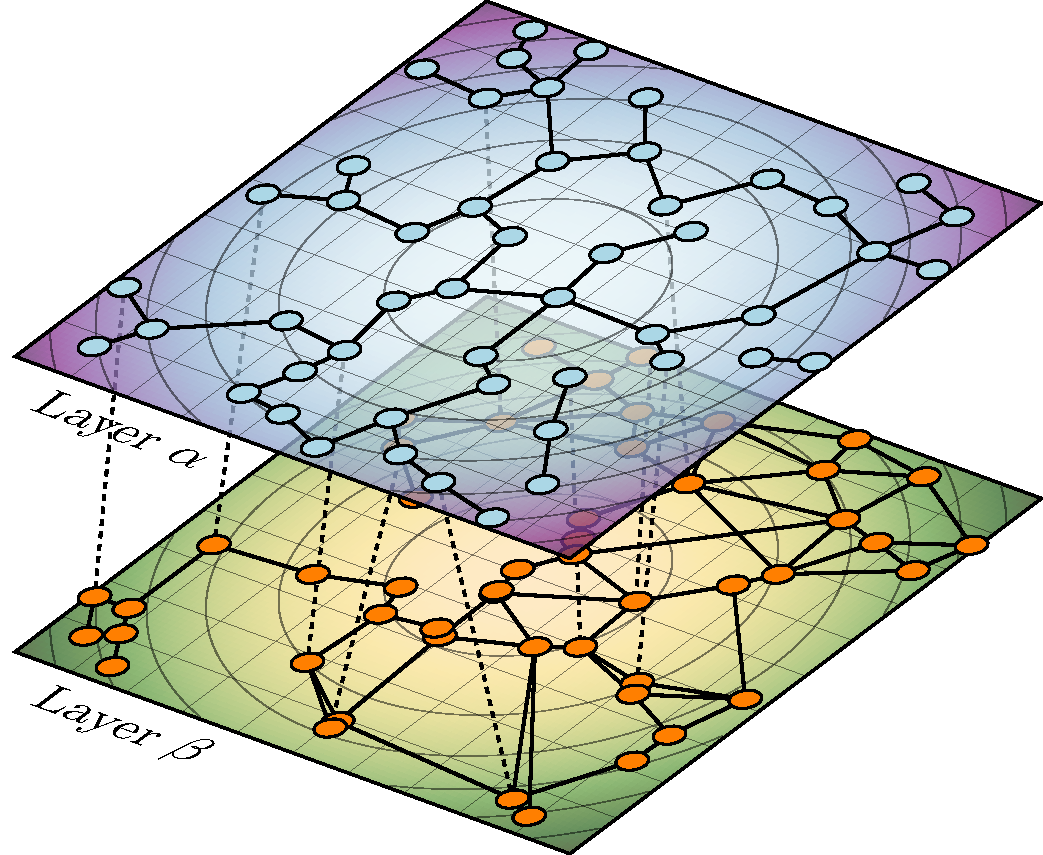
\includegraphics[bb=0 0 824 741]{../pictures/front.jpg} \\[5mm]
\else
        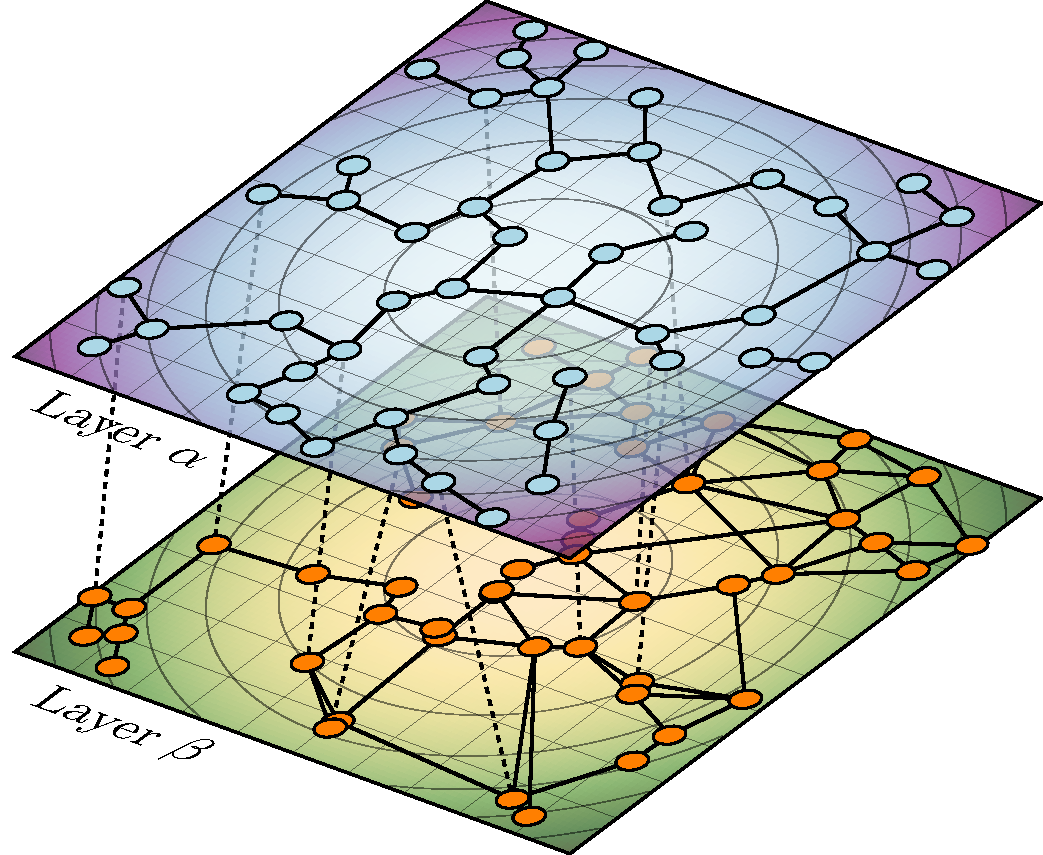
\includegraphics[width=.5\linewidth]{../pictures/front} \\[5mm]
\fi
        \small \textit{Documentation contacts:}\\[3mm]
        \small \begin{tabular}{lcr}
          Czech/Slovak & Petr Sojka & \email{sojka@fi.muni.cz} \\
                       & Janka Chleb\'\i kov\'a & \email{chlebikj (at) dcs.fmph.uniba.sk} \\
          English      & Karl Berry & \email{karl@freefriends.org} \\
          French       & Fabrice Popineau & \email{fabrice.popineau@supelec.fr} \\
          German       & Volker RW Schaa & \email{volker@dante.de} \\
          Polish       & Staszek Wawrykiewicz & \email{staw@gust.org.pl} \\
          Russian      & Boris Veytsman & \email{borisv@lk.net} \\
         \end{tabular}
         }

% comes out too close to the toc, and we know it's page one anyway.
\thispagestyle{empty}

\maketitle
\newpage

\begin{multicols}{2}
\tableofcontents
\listoftables
\end{multicols}

\section{Introduction}
\label{sec:intro}

This document describes the main features of the \TeXLive{} software
distribution\Dash a \TeX{} and \LaTeX{} distribution for Linux and other
Unix flavors, \MacOSX, and (32-bit) Windows systems.  (Warning: it is
not especially useful for older Mac or \acro{MS-DOS} systems.)  It
includes precompiled binaries for \TeX{}, \LaTeXe{}, \MF, \MP,
\BibTeX{} and many other programs; an extensive collection of
macros, fonts and documentation; and support for typesetting in many
different scripts from around the~world.

For the 2003 release, the last update of packages and programs was made
on September 3, 2003.  For newer versions, please consult \acro{CTAN},
\url{http://www.ctan.org}.

For a brief summary of the major changes in this edition of \TeXLive{},
see section~\ref{sec:history} on p.~\pageref{sec:history}.


\subsection{Basic usage of \protect\TeXLive{}}
\label{sec:basic}

You can use \TeXLive{} in three principal ways:

\begin{enumerate}

\item You can run \TeXLive{} directly from the distribution media
(except for the \pkgname{inst} distribution; see
section~\ref{sec:multiple-dist} on p.~\pageref{sec:multiple-dist}).
This takes almost no disk space, as you might expect, and gives you
immediate access to everything in \TeXLive{}.  Of course performance
will be worse than running on local disk, but you may well find it
acceptable.

\item You can install all or part of \TeXLive{} to a local disk.  This
is the most common use of \TeXLive.  You will need a minimum of 120
megabytes, 360 megabytes for a recommended system, and 800 megabytes for
a full system.

\item You can integrate a particular package or collection into your
existing \TeX{} system, either a \TeXLive{} system you installed earlier
or a different system.

\end{enumerate}

\noindent All of these are described in detail in the \acro{OS}-specific
installation sections.


\subsection{Getting help}
\label{sec:help}

The \TeX{} community is both active and friendly, and virtually all
serious questions end up getting answered.  However, the support is
informal, done by volunteers and casual readers, so it's especially
important that you do your homework before asking.  (If you prefer
commercial-style support, you can forego \TeXLive{} completely and
purchase a vendor's system; see
\url{http://tug.org/interest.html#vendors} for a list.)

Here is a list of resources, approximately in the order we recommend
using them:

\begin{description}
\item [\TeX{} \acro{FAQ}] The \TeX{} \acro{FAQ} is a huge compendium of
answers to all sorts of questions, from the most basic to the most
arcane.  It is included on \TeXLive{} in \OnCD{FAQ/english}, and is
available on the Internet through \url{http://faq.tug.org}.  Please
check here first.

\item [\TeX{} Catalogue] If you are specifically looking for a package,
font, program, etc., the \TeX{} Catalogue is the place to look.  It is a
huge list of all \TeX{}-related items.  See
\OnCD{texmf/doc/html/catalogue}, or
\url{http://www.ctan.org/tex-archive/help/Catalogue/catalogue.html}.

\item [\TeX{} Web Resources] This web page has many \TeX{}-related
links, in particular for numerous books, manuals, and articles on all
aspects of the system: \url{http://tug.org/interest.html}.

\item [support archives] The two principal forums for support are the
Usenet newsgroup \url{news:comp.text.tex} and the mailing list
\email{texhax@tug.org}.  So, their archives have thousands of past
questions and answers for your searching pleasure.  See
\url{http://groups.google.com/groups?group=comp.text.tex} and
\url{http://tug.org/mail-archives/texhax}, respectively.  A query on a
general web search engine, such as \url{http://google.com}, never hurts.

\item [posting questions] If you cannot find an answer, you can post to
\dirname{comp.text.tex} through Google or your newsreader, or through
email to \email{texhax@tug.org}.  But before you post, \emph{please}
read this \acro{FAQ} entry for advice on asking questions in such a way
that you're most likely to get an answer:
\url{http://www.tex.ac.uk/cgi-bin/texfaq2html?label=askquestion}.

\item [\TeXLive{} support] If you want to report a bug or have
suggestions or comments on the \TeXLive{} distribution, installation, or
documentation, the mailing list is \email{tex-live@tug.org}.  However,
if your question is about how to use a particular program included in
\TeXLive{}, you are better off writing to that program's maintainer or
mailing list.

\end{description}

The other side of the coin is helping others who have questions.  Both
\dirname{comp.text.tex} and \code{texhax} are open to anyone, so feel
free to join, start reading, and help out where you can.  Welcome to
\TeX{}!


\section{Structure of \protect\TeXLive}
\label{sec:struct-tl}

The main two installation scripts for Unix and \MacOSX{} are
\texttt{install-tl.sh} and \texttt{install-pkg.sh}.  We discuss them
in section \ref{sec:unix-install} on p.~\pageref{sec:unix-install}.
Here, we describe the structure and contents of \TeXLive{}.


\subsection{Multiple distributions: \protect\pkgname{live},
            \protect\pkgname{inst}, \protect\pkgname{demo}}
\label{sec:multiple-dist}

As of 2003, space limitations of \acro{CD-ROM} format have forced us to
divide \TeXLive{} into three distributions, as follows.

\begin{description}

\item [live] a complete, runnable system on \acro{DVD}; it is too large
for \acro{CD-ROM}.  (The \DVD{} also includes a snapshot of the \CTAN{}
repository, completely independent of \TeXLive{}.)

\item [inst(allable)] a complete system on \CD; in order to make it fit,
we had to compress everything we could.  Therefore, it is not possible
to run \TeX\ directly from the installable \CD, you have to install it to
disk (hence its name).  Installation is described in subsequent sections.
   
\item [demo] a live system runnable directly from \CD; in order to make
this fit, we omitted the very large collection of \acro{CJK} (Chinese,
Japanese, Korean) language support, support for typesetting music, some
less-commonly used fonts, and included executables only for Linux,
\MacOSX, and Windows systems.

\end{description}

\noindent You can tell which type of distribution you're in by looking
for a \texttt{00\var{type}.TL} file in this top-level directory.


\subsection{Top level directories}

Here is a brief listing and description of the top level directories in
the \TeXLive{} distribution.

\smallskip
\begin{tabular}{>{\ttfamily}lp{.8\hsize}}
bin     & The \TeX{} system programs, arranged by platform. \\
Books   & Examples from some of the books about \TeX\ (see
  \filename{Books/README}). \\
FAQ     & Current versions of major FAQ collections. \\
info    & A few manuals in \acro{GNU} Info format, where available. \\
\MacOSX & Supporting software for \MacOSX (see
  section~\ref{sec:mac-install} on p.~\pageref{sec:mac-install}). \\
man     & Unix man pages. \\
source  & The source of all programs, including the main \Webc{}
  \TeX{} and \MF{} distributions. These are stored in a
  \cmdname{bzip2}-compressed tar archive. \\
support & assorted auxiliary packages and programs.  These are
  \emph{not} installed by default.  This includes
  \cmdname{Ghostscript}, \cmdname{netpbm}, and assorted editors and
  \TeX\ shells. \\
texmf   & root of installed packages, fonts, config files, etc. \\
usergrps & Material about a few of the \TeX\ user groups.  (Visit
  \url{http://tug.org/usergroups.html} for a current list.) \\
xemtex  & The \cmdname{XEmacs} editor and other support programs for
  Windows (see section~\ref{sec:win-xemtex} on p.~\pageref{sec:win-xemtex}).
  These programs generally come pre-installed on Unix systems, or are
  at least easy to compile. \\
\end{tabular}


\subsection{Extensions to \TeX}
\label{sec:tex-extensions}

\TeXLive{} contains three extended versions of \TeX:

\begin{description}

\item [\eTeX] adds a small but powerful set of new primitives
\label{text:etex}
(related to macro expansion, character scanning, classes of marks,
additional debugging features, and more) and the \TeXXeT{} extensions
for bidirectional typesetting.  In default mode, \eTeX{} is 100\%
compatible with ordinary \TeX. See
\OnCD{texmf/doc/etex/base/etex_man.pdf}.  \eTeX{} is now the default for
\LaTeX{} and pdf\LaTeX{}.

\item [pdf\TeX] writes Acrobat PDF format as well as \dvi{}. The
\LaTeX{} \pkgname{hyperref} package has an option `\optname{pdftex}'
which turns on all the program features.  See
\OnCD{texmf/doc/pdftex/pdftex-l.pdf} and
\OnCD{texmf/doc/pdftex/base/example.tex}.

\item [\OMEGA\ (Omega)] based on Unicode (16-bit characters), thus
supports working with almost all the world's scripts simultaneously. It
also supports so-called `\OMEGA{} Translation Processes' (\acro{OTP}s),
for performing complex transformations on arbitrary input. See
\OnCD{texmf/doc/omega/base/doc-1.8.tex} (not completely up-to-date).

\end{description} 


\subsection{Other notable programs in \protect\TeXLive}

Here are a few other commonly-used programs included in \TeXLive{}:

\begin{cmddescription}

\item [bibtex] bibliography support.

\item [makeindex] index support.

\item [dvips] convert \dvi{} to \PS{}.

\item [xdvi] \dvi{} previewer for the X Window System.

\item [dvilj] HP LaserJet driver.

\item [dv2dt, dt2dv] convert \dvi{} to/from plain text.

\item [dviconcat, dviselect] cut and paste pages
from \dvi{} files.

\item [dvipdfm] convert \dvi{} to PDF, an alternative approach
to pdf\TeX\ (mentioned above).  See the \pkgname{ps4pdf} and
\pkgname{pdftricks} packages for still more alternatives.

\item [psselect, psnup, \ldots] \PS{}
utilities.

\item [lacheck] \LaTeX{} syntax checker.

\item [texexec] Con\TeX{}t and PDF processor.

\item [tex4ht] \TeX{} to HTML converter.  

\end{cmddescription}


\section{Unix installation}
\label{sec:unix-install}

As introduced in section~\ref{sec:basic} on p.~\pageref{sec:basic},
\TeXLive{} has three principal uses:

\begin{enumerate}
\item Run directly from media.
\item Install to disk.
\item Integrate a particular package or collection into your existing
\TeX{} installation.
\end{enumerate}

\noindent The following sections describes the Unix-specific procedures
for each of these.

\ifSingleColumn \begin{figure}[ht]\noindent \fi
\begin{warningbox}
\textbf{Warning: } The \TK{} \CD{}s and \DVD{} are in ISO 9660 (High Sierra)
format, \emph{with} Rock Ridge (and Joliet, for Windows)
extensions. Therefore, in order to take full advantage of the \TK{}
under Unix, your system needs to be able to use the Rock Ridge
extensions.  Please consult the documentation for your \cmdname{mount}
command to see how to do this.  If you have several different machines
on a local network, you may be able to mount the \CD{}s on one which
does support Rock Ridge, and use this with the others.

\leavevmode\quad Linux, Free\acro{BSD}, Sun, \acro{SGI} and
Alpha systems should be able to use the \CD{}s without problems. We
would appreciate receiving detailed advice from users on other systems
who succeed, for future versions of this documentation.

\leavevmode\quad
The discussion below assumes you have been able to mount
the \CD{}s with full Rock Ridge compatibility.
\end{warningbox}
\ifSingleColumn\end{figure}\fi


% 
\subsection{Running \protect\TeXLive{} directly from media (Unix)}

\def\runlive{% text repeated in windows section
It is possible to use the \TeX{} system directly from the \pkgname{demo}
\CD{} or the \pkgname{live} \DVD{}, without installing the distribution
to disk.  (Thus the name `\TeXLive', in fact.)  It is \emph{not}
possible to run \TeX{} directly from the \pkgname{inst} \CD (see
section~\ref{sec:multiple-dist} on p.~\pageref{sec:multiple-dist}).
}

Only Linux, \MacOSX, and Windows binaries are included on the demo \CD;
if you want to run live on other Unix systems, you'll need to use the
\DVD.

\def\startinst{% repeated in other subsections
To start, we must mount the \CD{} or \DVD{}, with Rock Ridge extensions
enabled.  The exact command to do this varies from system to system; the
following works under Linux, except the name of the device
(\filename{/dev/cdrom}, here) may vary. (All our examples will use
\texttt{>} as the shell prompt; user input is \underline{underlined}.)
\begin{alltt}
> \Ucom{mount -t iso9660 /dev/cdrom /mnt/cdrom}
\end{alltt}

\noindent Change the current directory to the mount point:
\begin{alltt}
> \Ucom{cd /mnt/cdrom}
\end{alltt}

\noindent Under \MacOSX, the directory is typically under
\dirname{/Volumes}, and the media will be mounted automatically.
}

\startinst

Run the installation script \filename{install-tl.sh}:
\begin{alltt}
> \Ucom{sh install-tl.sh}
Welcome to TeX Live...
\end{alltt}

\def\firstinstcommand{%
\noindent After various greeting messages and a list of the main menu
options, the installation will ask you to enter a command.  Do this by
typing the desired character and hitting return; don't type the angle
brackets.  Either uppercase or lowercase is ok; we'll use lowercase in
our examples.
}
\firstinstcommand

For running live, our first command will be \Ucom{d} and then the
subcommand \Ucom{1} to set directories.  Even in this case, we must
choose a directory on the local disk to place files that the \TeX{}
system itself generates, such as fonts and formats, and also to provide
a place for updated configuration files, if need be.  We'll use
\dirname{/usr/local/texmf-local} in this example. (If the default value
of \dirname{/usr/TeX} works for you, then you can skip this step.)
\begin{alltt}
Enter command: \Ucom{d}
Current directories setup:
<1>  TEXDIR:     /usr/TeX
...
Enter command: \Ucom{1}
New value for TEXDIR [/usr/TeX]: \Ucom{/usr/local/texmf-local}
...
Enter command: \Ucom{r}
\end{alltt}

\noindent Back at the main menu, our second and last command is
\Ucom{r}, to set up for running live off the media without installing
to disk:
\begin{alltt}
Enter command: \Ucom{r}
Preparing destination directories...
...
Welcome to the TeX Live system!
>
\end{alltt}

\noindent And we are back at the system prompt, as shown.

Next, it is necessary to alter two environment variables:
\envname{PATH}, to an architecture-dependent value (so that we can run
the programs), and \envname{VARTEXMF}, to the value specified above.  See
table~\ref{tab:archlist} for a list of the architecture names for the
different systems, and whether they are available on the \pkgname{demo}
\CD.  All systems are available in the \pkgname{inst} and \pkgname{live}
distributions.  (In addition to the version-specific names listed here,
there are generic names without the version numbers.  For instance,
\dirname{sparc-solaris} links to \dirname{sparc-solaris2.7}.  The
generic names can be used to protect against the version numbers
changing in the future, if you wish.)

\def\runtexconfig{%
After the main installation has completed, and environment variables
have been set, the next step is to run \cmdname{texconfig} to customize
your installation for your needs.  This is explained in
section~\ref{sec:texconfig}, p.~\pageref{sec:texconfig}.
}
\runtexconfig

\begin{table*}[ht]
\caption{Supported system architectures.}
\label{tab:archlist}
\begin{tabular}{>{\ttfamily}lll}
alpha-linux	   & HP Alpha Linux   & \\
alphaev5-osf4.0d   & HP Alphaev5 OSF  & \\
%hppa2.0-hpux10.20  & HP9000 HPUX 10.20	  & \\
i386-freebsd4.8    & Intel x86 FreeBSD    & \\
i386-linux         & Intel x86 GNU/Linux  & demo \CD\\
i386-openbsd3.3    & Intel x86 OpenBSD    & \\
i386-solaris2.8    & Intel x86 Solaris    & \\
mips-irix6.5       & SGI IRIX             & \\
powerpc-aix4.3.3.0 & IBM RS/6000 AIX      & \\
powerpc-darwin6.3  & \MacOSX              & demo \CD\\
sparc-solaris2.7   & Sun Sparc Solaris    & \\
sparc64-linux      & Sun Sparc Linux      & \\
win32		   & Windows (32-bit)     & demo \CD\\
\hline
\end{tabular}
\end{table*}

\label{text:path}
The syntax for setting the environment variables, and the initialization
file to put them in, depends on the shell you use.  If you use a
Bourne-compatible shell (\cmdname{sh}, \cmdname{bash}, \cmdname{ksh}, et
al.), put the following into your \filename{$HOME/.profile} file:
\begin{alltt}
PATH=/mnt/cdrom/bin/\Ucom{\emph{archname}}:$PATH; export PATH
VARTEXMF=/usr/local/texmf-local/texmf-var; export VARTEXMF
\end{alltt}

\noindent For C shell-compatible shells (csh, tcsh), put the following
into your \filename{$HOME/.cshrc} file:
\begin{alltt}
setenv PATH /mnt/cdrom/bin/\Ucom{\emph{archname}}:$PATH
setenv VARTEXMF /usr/local/texmf-local/texmf-var
\end{alltt}

\def\donewithinst{%
\noindent Then log out, log back in, and test your installation
(see section~\ref{sec:test-install} on p.~\pageref{sec:test-install}).
}
\donewithinst

\def\ifindoubt{%
If in doubt, please ask any local system gurus to help you with
problems; for example, the way to mount the \TeXLive{} media, which
directory or directories to use, and precise details of the changes to
your personal initialization files can and do vary from site to site.
}
\ifindoubt


% 
\subsection{Installing \protect\TeXLive{} to disk}
\label{sec:unix-install-disk}

It is possible, indeed typical, to install the \TeX{} system from the
\TeXLive{} to disk.  This can be done either from the \pkgname{live}
\DVD, or the \pkgname{inst} \CD.  It can also be done from the
\pkgname{demo} \CD, if you don't need the omitted packages or systems.
(See section~\ref{sec:multiple-dist} on p.~\pageref{sec:multiple-dist}
for an explanation of the different distributions.)

\startinst

Run the installation script \filename{install-tl.sh}:
\begin{alltt}
> \Ucom{sh install-tl.sh}
Welcome to TeX Live...
\end{alltt}

\firstinstcommand

Here is an introductory list of the options in the main menu.  The order
in which you select the options makes little difference, except that
\Ucom{i} must be last.  It's reasonable to go through them in the
order presented~here.

% apparently here.sty [H] doesn't support table*.
\begin{table}[H]
\caption{Main menu options for the installation.}
\label{tab:main-menu-options}
\begin{tabular}{>{\ttfamily}ll}
p & The system you are running on.\\
b & The architectures to install binaries for.\\
s & The base installation scheme to use (minimal, recommended,
          full, etc.)\\
c & Override the installation scheme for individual collections.\\
l & Override for language collections.\\
d & Directories in which to install.\\
o & General options.\\
i & Perform the installation.\\
\end{tabular}
\end{table}

Here are further details on each option.

\textbf{\optname{p} -- Current platform.}  Since the installation script
automatically guesses which platform you're running on, this is
generally unnecessary to override.  It's there in case the automatic
detection fails.

\textbf{\optname{b} -- Binary architectures.}  By default, only the
binaries for your current platform will be installed.  From this menu,
you can select installation of binaries for other architectures as well
(or not install the current platforms).  This is often useful if you
are sharing a \TeX\ tree across a network of heterogenous machines.  For
a list of the supported architectures, see table~\ref{tab:archlist},
p.~\pageref{tab:archlist}.

\textbf{\optname{s} -- Base installation scheme.}  From this menu, you
can choose an overall common set of packages.  The default is a
recommended set for typical needs, but you can also choose a basic set
to conserve disk space, or a full set to get absolutely everything.  The
\pkgname{Live} scheme is used for creating the \TeXLive{}
\pkgname{demo} distribution itself, and isn't generally useful to select
for a particular site.  There are also specific sets for Omega and
\acro{XML} users.

\textbf{\optname{c} -- Individual collections.}  From this menu, you can
override the basic scheme's choice of which collections to install.
Each collection\Dash TeX macro files, Metafont font families, and so
on\Dash consists of several packages.  In this menu, selection letters
are case-sensitive.

\textbf{\optname{l} -- Language collections}.  This menu has the same
basic functionality as \Ucom{c}, to override collection choices.  In
this case, the collections are specifically for different languages.
Selection letters are case-sensitive here.  Here is a list of the
language collections in \TeXLive:

% xx really should generate list from texmf/tpm/collection/tex-lang*
% a la install-tl.sh.
\begin{tabbing}
\hspace{.25\linewidth} \=
\hspace{.25\linewidth} \=
\hspace{.25\linewidth} \=
\hspace{.25\linewidth} \kill
  (some) African scripts \>
  Armenian \>
  Chinese,Japanese,Korean \>
Croatian \\
  Cyrillic \>
  Czech/Slovak \>
  Danish \>
Dutch \\
  Finnish \>
  French \>
  German \>
Greek \\
  Hungarian \>
  Indic \>
  Italian \>
Latin \\
  Manju \>
  Mongolian \>
  Norwegian \>
Polish \\
  Portuguese \>
  Spanish \>
  Swedish \>
Tibetan \\
  \acro{UK} English \>
Vietnamese \\
\end{tabbing}

\noindent Language collections typically includes fonts, macros,
hyphenation patterns, and other support files.  (For instance,
\pkgname{frenchle.sty} is installed if you select the \optname{French}
collection.)  In addition, installing a language collection will alter
the \filename{language.dat} configuration file controlling which
hyphenations are loaded.

\textbf{\optname{d} -- Installation directories}.  Three directories can
be changed here:
\label{text:instdir}

\begin{ttdescription}
\item [TEXDIR] By default, the top-level directory under which
everything else will be installed.  The default value is
\dirname{/usr/TeX}, and is often changed.  For example, changing to a
value such as \dirname{/usr/local/texlive2003} would make it possible to
keep different releases of \TeXLive{} separate.  You may then wish to
make \dirname{/usr/local/texlive} a symbolic link, after testing the new
release.

Under \MacOSX, the usual frontends look for \TeX{} in
\dirname{/usr/local/teTeX}, so you may wish to install \TeXLive{} there.

\item [TEXMFLOCAL] This tree is where the \TeX{} system scripts install
non-version-specific files, primarily fonts.  The default value is
\dirname{TEXDIR/texmf-local}.  It's also the recommended location to put
any local packages or configuration settings.  Therefore, it's desirable
to change it to a location independent of the current \TeXLive{}
release; for example, \dirname{/usr/local/texmf-local}.

\item [VARTEXMF] This tree is where the scripts install files that
\emph{are} version-specific, primarily format files and the
configuration files which are modified by \cmdname{texconfig} (see
section~\ref{sec:texconfig}, p.~\pageref{sec:texconfig}).  The default
value is \dirname{TEXDIR/texmf-var}, and there's generally no reason to
change it.

\end{ttdescription}

\textbf{\optname{o} - General options.}  From this menu, you can select
three general options affecting the installation:

\begin{ttdescription}
\item [a] Specify an alternate directory for generated fonts.
The default is to use the \envname{VARTEXMF} tree, as explained above.
Setting this is useful if you plan to mount the main tree read-only, and
therefore another location (perhaps machine-specific) must be used for
dynamically created fonts.

\item [l] Create symbolic links for the binaries, man pages,
and/or \acro{GNU} Info files in other locations.  For example, you may
wish to make the man pages available under \dirname{/usr/local/man} and
the Info files available under \dirname{/usr/local/info}.  (Of course
you need appropriate privileges to write in the specified directories.)

\item [d] Skip installation of the font/macro documentation tree.
This is useful to save space, or if you've previously installed the
documentation elsewhere.

\item [s] Skip installation of the main font/macro source
tree.  This is useful if you are arranging to share that tree between
machines and/or architectures in some other way, such as \acro{NFS} or
\cmdname{automount}.

\end{ttdescription}

\textbf{i - Perform installation.}  When you're satisfied with your
configuration options, enter \Ucom{i} to actually do the installation
from the media to your chosen locations.

The last step is to include the architecture-specific subdirectory of
\dirname{TEXDIR/bin} in your
\envname{PATH}, so the newly-installed programs can be found.  The
architecture names are listed in table~\ref{tab:archlist},
p.~\pageref{tab:archlist}, or you can simply list the directory
\dirname{TEXDIR/bin}.

The syntax for doing this, and the initialization file to put it in,
depends on the shell you use.  If you use a Bourne-compatible shell
(\cmdname{sh}, \cmdname{bash}, \cmdname{ksh}, et al.), put the following
into your \filename{$HOME/.profile} file:
\begin{alltt}
PATH=/\Ucom{\emph{TEXDIR}}/bin/\Ucom{\emph{archname}}:$PATH; export PATH
\end{alltt}

\noindent For C shell-compatible shells (\cmdname{csh}, \cmdname{tcsh}),
put the following into your \filename{$HOME/.cshrc} file:
\begin{alltt}
setenv PATH /\Ucom{\emph{TEXDIR}}/bin/\Ucom{\emph{archname}}:$PATH
\end{alltt}

\runtexconfig

Here is a brief annotated example which selects a full installation,
with binaries for the current system only, with directory changes as
recommended above.  The prompts and \acro{RETURN} keys are omitted for
brevity.

\begin{alltt}
> \Ucom{sh install-tl.sh}
\Ucom{s} \Ucom{b} \Ucom{r}                     # scheme, full, return to main
\Ucom{d}                         # change directories
\Ucom{1} \Ucom{/usr/local/texlive2003}  # top-level dir
\Ucom{2} \Ucom{/usr/local/texmf-local}  # TEXMFLOCAL outside TEXDIR
\Ucom{r}                         # return to main
\Ucom{i}                         # perform installation
> \Ucom{texconfig} ...
# New PATH, assuming Linux:
> \Ucom{PATH=/usr/local/texlive2003/bin/i386-linux:$PATH; export PATH}
\end{alltt}

\ifindoubt


% 
\subsection{Installing individual packages to disk}

You can add individual packages or collections from the current
distribution to an existing non-\TeXLive{} setup, or an earlier
\TeXLive{} installation.  You can do this from the \pkgname{demo} \CD{}
or the \pkgname{live} \DVD{}, but \emph{not} from the \pkgname{inst}
\CD.  (See section~\ref{sec:multiple-dist} on
p.~\pageref{sec:multiple-dist}.)

\startinst

Run the installation script \filename{install-pkg.sh} (not
\filename{install-tl.sh}, which is intended for complete installations
only):
\begin{alltt}
> \Ucom{sh install-pkg.sh \emph{options}}
\end{alltt}

This first set of options controls what gets read:

\begin{ttdescription}
\item [-{}-package=\emph{pkgname}] The individual package to work on.

\item [-{}-collection=\emph{colname}] The individual collection to work on.

\item [-{}-nodoc] Exclude documentation files from the operation.

\item [-{}-nosrc] Exclude source files from the operation.

\item [-{}-cddir=\emph{dir}] Source directory to read from; defaults
to the current directory.  If you followed the instructions above, that
will be the distribution directory, and won't need to be changed.

\item [-{}-listdir=\emph{dir}] The so-called `lists' directory within
\emph{cddir} from which to read the package information.  The default is
\texttt{\emph{cddir}/texmf/tpm/lists}; the only reason to change it is
if you're making changes to \TeXLive{} yourself.

\end{ttdescription}

What actually happens is controlled by the following options.  If
neither of these are specified, the default action is to install the
selected files.  The main destination tree is found by expanding
\envname{\$TEXMFMAIN} with \cmdname{kpsewhich}.  You can override it by
setting either the environment variable \envname{TEXMFMAIN} or
\envname{TEXMF}.

\begin{ttdescription}
\item [-{}-listonly] List the files that would be installed, but don't
actually install anything.

\item [-{}-archive=\emph{tarfile}] Instead of installing the files into
the \TeX{} system, make a \cmdname{tar} archive.

\end{ttdescription}

Additional options:

\begin{ttdescription}

\item [-{}-config] After installation, run \code{texconfig init}.

\item [-{}-nohash] After installation, don't run \cmdname{mktexlsr} to
rebuild the filename database.

\item [-{}-verbose] Give more information as the script runs.

\end{ttdescription}

Here are some usage examples:

\begin{enumerate}

\item To see the files in the package \pkgname{fancyhdr} without
installing it:

\begin{alltt}
\ifSingleColumn> \Ucom{sh install-pkg.sh --package=fancyhdr --listonly}
\else> \Ucom{sh install-pkg.sh --package=fancyhdr \bs}
>                           \Ucom{--listonly}
\fi{}
texmf/doc/latex/fancyhdr/README
texmf/doc/latex/fancyhdr/fancyhdr.dvi
texmf/doc/latex/fancyhdr/fancyhdr.pdf
...
\end{alltt}

\item Install the \LaTeX{} package \pkgname{natbib}:
\begin{alltt}
> \Ucom{sh install-pkg.sh --package=natbib}
\end{alltt}

\item Install the \LaTeX{} package \pkgname{alg} without source files or
documentation:
\begin{alltt}
\ifSingleColumn> \Ucom{sh install-pkg.sh  --package=alg --nosrc --nodoc}
\else> \Ucom{sh install-pkg.sh  -{}-package=alg \bs}
>                  \Ucom{-{}-nosrc -{}-nodoc}
\fi\end{alltt}

\item Install all the packages in the collection of additional
plain \TeX\ macros:
\begin{alltt}
> \Ucom{sh install-pkg.sh --collection=tex-plainextra}
\end{alltt}

\item Write all files in the \pkgname{pstricks} package to a
\cmdname{tar} file in \path|/tmp|:
\begin{alltt}
\ifSingleColumn> \Ucom{sh install-pkg.sh --package=pstricks --archive=/tmp/pstricks.tar}
\else
> \Ucom{sh install-pkg.sh -{}-package=pstricks \bs}
>          \Ucom{-{}-archive=/tmp/pstricks.tar}
\fi\end{alltt}

\end{enumerate}

\ifindoubt


% 
\section{Post-installation}
\label{sec:postinstall}

After the main installation is done, for any operating system, the
remaining steps are to configure the system for your local needs, and
perform some basic tests.

Another sort of post-installation is to acquire packages, fonts, or
programs that were not included in \TeXLive{}.  The basic idea is to
install such additions in the \envname{TEXMFLOCAL} tree (if you
installed to disk), or \envname{VARTEXMF} (if you are running live).
See ``Installation directories'' on p.~\pageref{text:instdir}.

Unfortunately, the details can vary widely, and so we do not attempt to
address them here.  Please see
\url{http://www.ctan.org/tex-archive/info/beginlatex/html/chapter5.html#pkginst}
for a good description, and 
\url{http://www.ctan.org/tex-archive/info/Type1fonts} for font creation
and installation information in particular.


\subsection{The \protect\cmdname{texconfig} program}
\label{sec:texconfig}

At any time after installation, you can and should use the program
\cmdname{texconfig} to configure the system to fit your local needs.  It
is installed in the architecture-specific subdirectory
\texttt{TEXDIR/bin/\emph{arch}} along with everything else.

If you run it without arguments, it will enter full-screen mode and
allow you to view and change options interactively.

You can also run it with various command-line options.  Here are some of
the most commonly used:

\begin{ttdescription}

\item [texconfig dvips paper letter] Set default paper size for
\cmdname{dvips} to be letter-size.

\item [texconfig xdvi us] Likewise, for \cmdname{xdvi}.

\item [texconfig rehash] Update all the \TeX{} system filename databases.

\item [texconfig faq] Show the \teTeX{} \acro{FAQ}.
(See also the main \TeX{} \acro{FAQ} in the \dirname{FAQ} subdirectory
of \TeXLive.)

\item [texconfig help] Output help information.

\end{ttdescription}

Of course, \cmdname{texconfig} only supports changing a few of the many
options and configuration parameters in a \TeX{} system.  The main
configuration file for the base \Webc{} programs is named
\filename{texmf.cnf}.  You can find its location by running
\samp{kpsewhich texmf.cnf}; it contains many comments explaining the
default settings and useful alternatives.


\subsection{Testing the installation}
\label{sec:test-install}

After installing \TeXLive{} as best you can, you naturally want to test
it out, so you can start creating beautiful documents and/or fonts.

This section gives some basic procedures for testing that the new system
is functional.  We described the Unix commands; under \MacOSX{} and
Windows, you're more likely to run the tests through a graphical
interface, but the principles are the same.

\begin{enumerate}

\item Make sure that you can run the \cmdname{tex} program in the first
place:

\begin{alltt}
> \Ucom{tex -{}-version}
TeX (Web2c 7.5.2) 3.141592
kpathsea version 3.5.2
Copyright (C) 1997-2003 D.E. Knuth.
...
\end{alltt}
If this comes back with `command not found' instead of version and
copyright information, most likely you don't have the correct
\dirname{bin} subdirectory in your \envname{PATH}.  See
the environment-setting information on p.~\pageref{text:path}.

\item Process a basic \LaTeX{} file:
\begin{alltt}
> \Ucom{latex sample2e.tex}
>TeX (Web2c 7.5.2) 3.141592
...
Output written on sample2e.dvi (3 pages, 7256 bytes).
Transcript written on sample2e.log.
\end{alltt}
If this fails to find \filename{sample2e.tex} or other files, perhaps
you have interference from old environment variables or configuration
files.  For a deep analysis, you can always ask \TeX{} to report on
exactly what it is searching for, and finding; see ``Debugging actions''
on page~\pageref{Debugging}.

\item Preview the result online:
\begin{alltt}
> \Ucom{xdvi sample2e.dvi}
\end{alltt}
Under Windows, the analogous command is \cmdname{windvi}.  You should
see a new window with a nice document explaining some of the basics of
\LaTeX{}.  (Well worth reading, if you're new to the system.)  You do
have to be running under X for \cmdname{xdvi} to work; if you're not, or
your \envname{DISPLAY} environment variable is set incorrectly, you'll
get an error \samp{Can't open display}.

\item Create a \PS{} file for printing or display:
\begin{alltt}
> \Ucom{dvips sample2e.dvi -o sample2e.ps}
\end{alltt}

\item Create a \acro{PDF} file instead of \dvi{}; this processes the
\filename{.tex} file and writes \acro{PDF} directly:
\begin{alltt}
> \Ucom{pdflatex sample2e.tex}
\end{alltt}

\item Preview the \acro{PDF} file:
\begin{alltt}
> \Ucom{gv sample2e.pdf}
\textrm{or:}
> \Ucom{xpdf sample2e.pdf}
\end{alltt}
Unfortunately neither \cmdname{gv} nor \cmdname{xpdf} are currently
included in \TeXLive{}, so you must install them separately.  See
\url{http://wwwthep.physik.uni-mainz.de/~plass/gv} and
\url{http://www.foolabs.com/xpdf}, respectively.

\item Other standard test files you may find useful:

\begin{ttdescription}
\item [docstrip.tex] Produce \TeX{} source or documentation from a
\samp{.dtx} file.
\item [small2e.tex] A simpler document than \filename{sample2e}, to
reduce the input size if you're having troubles.
\item [testpage.tex] Test if your printer introduces any offsets.
\item [nfssfont.tex] For printing font tables and tests.
\item [testfont.tex] Also for font tables, but using plain \TeX{}.
\item [story.tex] The most canonical (plain) \TeX{} test file of all.
You must type \samp{\bs bye} to the \code{*} prompt after \samp{tex
story.tex}.
\end{ttdescription}
You can process these in the same way as we did with
\filename{sample2e.tex}.

\end{enumerate}

If you are new to \TeX{}, or otherwise need help with actually
constructing \TeX{} or \LaTeX{} documents, please visit
\url{http://tug.org/begin.html}.  We especially recommend the
\textsl{Formatting Information} manual by Peter Flynn, available at
\url{http://www.ctan.org/tex-archive/documentation/beginlatex}.


\section{\MacOSX{} installation}
\label{sec:mac-install}

\TeXLive{} supports \MacOSX, but no prior Macintosh versions.  (If you
are running an older Mac version, you can view the files by installing
the Joliet system extension available from
\url{http://www.tempel.org/joliet}; however, the \TeXLive{} binaries
will not run.)

Installation of \TeX{} under \MacOSX{} can be done in two ways:

\begin{enumerate}
\item With the \filename{install*} scripts, as with Unix.
\item With the \cmdname{i-Installer} included in
\filename{MacOSX/II2.dmg}.
\end{enumerate}

\noindent Each of these is described in a following section.

In addition, typical use of \TeX{} under \MacOSX\ goes through a
\emph{frontend}.  This is also described below.


\subsection{\protect\cmdname{i-Installer}: Internet installation}
\label{sec:i-Installer}

The \cmdname{i-Installer} is included in the \TeXLive{} distribution as
an alternative to normal installation.  It does not use the contents of
the \TeXLive{} distribution at all; instead, the system (approximately
70 megabytes) is downloaded over the Internet.

One advantage of \cmdname{i-Installer} is that it makes updates
relatively painless.  If you are interested, please see the
\cmdname{i-Installer} \TeX{} home page at \url{http://www.rna.nl/tex.html}.

To use it, mount \filename{./MacOSX/II2.dmg}.  Read the documentation,
launch it, and install at least \emph{TeX Foundation} and \emph{TeX
Programs}. The first will finish without configuration, as soon as the
second is installed you will be presented with a graphical interface to
setting up your \TeX{} system.

The \cmdname{i-Installer} distribution uses the \teTeX{} \dirname{texmf}
tree with some additions. Due to differences between \TeXLive{} and
\teTeX{} you cannot update a \TeXLive{} installation with an
\cmdname{i-Installer} \emph{TeX Programs} i-Package.


\subsection{\protect\cmdname{install*.sh}: \protect\TeXLive{} installation}

In order to run the installation scripts under \MacOSX, you need to have
the \cmdname{bash} shell installed.  If you are running \MacOSX~10.2
or later, you have \cmdname{bash}, and can proceed.  If you're running
an earlier \MacOSX{} version, however, the default shell is
\cmdname{zsh}, which won't work; please see the
subsection~\ref{sec:mac-bash} (p.~\pageref{sec:mac-bash}) below for
instructions on installing bash \cmdname{bash}.

Once you have \cmdname{bash}, the Unix installation documentation in the
previous section can be followed.  See section~\ref{sec:unix-install} on
p.~\pageref{sec:unix-install}; \MacOSX-specific notes are included where
needed.


\subsection{\MacOSX{} frontends}

Using \TeX{} on a Macintosh typically goes through a front end program,
comprising an execution shell, editor, previewer, and other facilities.
Here are the principal frontends:

\begin{cmddescription}
\item [TeXShop] Included in \TeXLive{} as
\filename{./MacOSX/texshop.dmg}.  See
\url{http://www.uoregon.edu/~koch/texshop/texshop.html}.

\item [ITeXMac] Included in \TeXLive{} as
\filename{./MacOSX/iTeXMac-*.dmg}.  See
\url{http://itexmac.sourceforge.net}.

\item [Mac-emacs] A port of Emacs to \MacOSX{}, integrating
\pkgname{AucTeX}.  See \url{http://www.cs.man.ac.uk/~franconi/mac-emacs}.

\end{cmddescription}

The frontends use \dirname{/usr/local/teTeX} as the default location;
therefore, you must either install \TeXLive{} there, or change the
configuration of the frontend.


\subsection{\cmdname{bash} installation for older \MacOSX{} versions}
\label{sec:mac-bash}

\MacOSX{} versions 10.1 and earlier do not include \cmdname{bash} by
default, and the default shell does not run the \TeXLive{} installation
scripts properly.  This section explains how to install \cmdname{bash}.

First, check if bash is already installed.  `Launch Terminal'
(\filename{/Applications/utilities/Terminal}) and type \code{rehash;
which bash}.  If the answer is a filename (for example,
\code{/bin/bash}), then \cmdname{bash} is already installed, and you're done
here; go back to the main installation instructions.
If the answer is \code{bash: command not found}, proceed here.

There are two ways to install \cmdname{bash} if you need it\Dash via the
\acro{GUI} or via command line.

To install via \acro{GUI}, double-click the \filename{MacOSX/bash.dmg}
file in \TeXLive{}.  The disk image (volume) will be mounted.  Then
start the \cmdname{i-Installer} application on that volume. You will be
asked to authenticate; if you have never seen that before, you might not
have enough privileges to install. Just enter your own user name and
password. Hit install. Bash will be installed on your system.

To install via command line:
\begin{enumerate}
\item ensure you have admin privileges: log in as the
\code{admin} user, the System Administrator, a user with Admin
privileges, using \cmdname{sudo}, etc.

\item copy \filename{MacOSX/bash.tar.gz} from the \TeXLive{}
distribution to your home directory.

\item Launch Terminal, and run:
\begin{alltt}
(cd /usr/local/; sudo tar xvzf ~/bash.tar.gz)
\end{alltt}
You'll be asked for your password, and then \cmdname{bash} will be
installed.

\item Quit Terminal.

\end{enumerate}

After using either installation method, be sure to recheck that
\cmdname{bash} is installed with \code{rehash; which bash} in a new
Terminal window.


\section{Windows installation}
\label{sec:win-install}

\TeXLive{} can be installed on systems running Windows 9x, \acro{ME},
\acro{NT}, \acro{2K} or \acro{XP}.  Older versions of Windows (3.1x)
and \acro{MS-DOS} are not supported.

It is necessary to have your Windows set up so that it uses the
Microsoft Joliet extensions for reading \CD{}s; simply look at the \CD{}
in Explorer and see whether it shows long, mixed-case, file names. If it
does not, you must install the Joliet extensions.

The Windows \TeX{} system included in \TeXLive{} is no more and no less
than the \fpTeX{} distribution.  It includes a \texttt{dvi} previewer,
\textsf{Windvi}, which is similar in usage to the established Unix
\textsf{xdvi}. The documentation can be found in
\OnCD{texmf/doc/html/windvi/windvi.html}.

\subsection{The \texttt{TeXLive.exe} program}

\begin{figure*}
 \begin{center}
  \ifnum \Status=1
    \includegraphics[width=.7\textwidth]{../pictures/Welcome-to-TeXLive}
  \else
    \ifnum \Status=2
        \includegraphics[bb=0 0 551 534]{../pictures/Welcome-to-TeXLive.jpg}
    \else
        \includegraphics[width=.7\textwidth]{../pictures/Welcome-to-TeXLive}
    \fi
  \fi
 \end{center}
 \caption{``Welcome to \TeXLive'' window}\label{graph:welcome}
\end{figure*}

If your computer is configured to let the \CD{} autostart, then a dialog
box with a menu bar will popup on the screen, and you will have several
choices from there:

\begin{itemize}
\item Install \TeX{} on your hard disk
\item Do maintenance on your \TeX{} system.
\item Remove the \TeX{} system.
\item Use \TeX{} off the \TeXLive{} \CD{} or \DVD{}.
\item Browse documentation: \TeXLive{} documentation, TUG web
  pages, \fpTeX web pages.
\item Run the \cmdname{TeXdocTK} application to find specific documentation.
\end{itemize}

If your \CD{} does not autostart, you can explicitly run the program
by double clicking on \path|bin/win32/TeXLive.exe| on the \CD{} from
the explorer window.

\subsection{Running \protect\TeXLive{} directly from media (Windows)}

\runlive

To run live under Windows, from the menu, chose \verb|Explore CD-Rom|, then  
\verb|Run TeX off CD-Rom|. This will launch the \cmdname{XEmacs} editor.
  
%% To run live under Windows, do the following:

%% \begin{enumerate}
%% \item from the menu, chose \verb|Explore CD-Rom|, then  
%%   \verb|Run TeX off CD-Rom|, that will launch the \cmdname{XEmacs} editor.
  
%%   This program needs to be a \TeX{} oriented editor. It must be able
%%   to run the \TeX{} compiler, previewer and any other needed tool. If
%%   you don't have one already installed on your system, you can install
%%   one from the \CD{}, details section~{\ref{sec:texlive-install}}.

%%   \emph{There is no way  we can guess if the program you will
%%     select is actually a text editor, so be careful}.
%%   Here is a list of frequently used \TeX{} editors:
%% \begin{center}
%%   \begin{tabular}[H]{ll}
%%     GNU Emacs & \path|c:\Program Files\NTEmacs\bin\runemacs.exe| \\
%%     XEmacs & \path|c:\Program Files\XEmacs\XEmacs-21.2\i586-pc-win32\xemacs.exe| \\
%%     WinShell & \path|c:\Program Files\WinShell\WinShell.exe| \\
%%     WinEdt & \path|c:\Program Files\WinEdt Team\WinEdt\WinEdt.exe|\\
%%     TeXnicCenter & \path|c:\Program Files\TeXnicCenter\TEXCNTR.exe|
%%   \end{tabular}
%% \end{center}
%%  The program
%%   selected will be memorized as the editor to use for future runs.

%% \item from the menu, chose \verb|Explore CD-Rom|, then  
%%   \verb|Run TeX off CD-Rom|. The environment will be modified, a small
%%   temporary directory created and some configuration files copied
%%   there. Then, the selected editor selected will be launched, and you
%%   will be able to type in some text, let \TeX{} typeset it and the
%%   view it or print it.

%%   If Ghostscript is not detected on your machine, you will be warned
%%   that rendering your DVI files might fail. You can install it from
%%   the \path|Install|, \path|Support| menu item. See
%%   section~\ref{sec:texlive-install} for details.

%% \item you can select a different text editor any time you want.

%% \item if you chose \verb|Cleanup CD-Rom setup|, everything \TeX{}
%%   needed will be  removed, comprised the selection of your text
%%   editor, but not the extra packages you may have downloaded and
%%   installed. If you installed \cmdname{WinShell} or \cmdname{NTEmacs}, 
%% they won't be removed.
%% \end{enumerate}

XEmacs startup file will set the environment variables needed. XEmacs will also
setup a temporary \acro{TDS} compliant texmf tree in the temporary area of your
computer.  It is needed to store files that may be built on the fly, such as
\path|pk| bitmap fonts, or format files.  Configuration files are copied from
the \CD{} to this texmf tree, so that you can edit them if needed.  The
\path|ls-R| database is computed for this texmf tree. The AUC-\TeX{} mode will
be entered  Whenever you will visit or create a \TeX{} file, providing all the
bells and whistles for \TeX{} support XEmacs is capable of.

If you run 'M-x shell' within XEmacs, then you will have access to all the TeXLive
tools from the command line provided by XEmacs.

\smallskip {\small\noindent \textbf{[For advanced users:]} You can also
  use the small batch file \path|mkloctex.bat| to be called in a
  directory \path|bin\win32| of the \CD.  From the Start menu select
  `Run', then browse the \acro{CD} drive and select
  \path|mkloctex.bat|. Before starting it, you should add two parameters
  separated by a space: the letter of your \acro{CD} drive and the
  letter of the drive where you want to install the \TeX\ directory.
  The whole line should read, e.g., \verb+d:\bin\win32\mkloctex.bat d c+.
  When installation is complete, please read carefully the information
  on screen. If you are running Windows 9x/\acro{ME}, then you will have to
  restart Windows.}

\subsection{Support packages for Windows}
\label{sec:win-xemtex}

To be complete, a \TeXLive installation needs support packages that are not
commonly found on a Windows machine.
Many scripts are written using the Perl language. Some important tools require
the Ghostscript \PS{} interpreter to render or to convert files. A graphic
file toolbox is also needed in some cases. Last but not least, a \TeX-oriented
editor makes it easy to type in your \TeX{} files.

All these tools are quite easy to find for Windows, but in order to try to make
your life even easier, we have put such a set of tools on \TeXLive:
\begin{itemize}
\item \cmdname{Ghostscript} 7.07
\item a minimal \cmdname{Perl} 5.8, sufficient to run all the \TeXLive{}
Perl scripts
\item a subset of \cmdname{ImageMagick} 5.5.6
\item the \cmdname{ISpell} checker
\item \cmdname{XEmacs} 21.5.14 with a selection of packages to support
\TeX{} typesetting.
\end{itemize}

These packages should be installed only all at once.  The bundle is
known as the \XEmTeX{} bundle. 

If you didn't install \XEmTeX{}, \cmdname{Perl} and \cmdname{Ghostscript} are
installed anyway if they are not detected on your machine. This is because they are
required by many important tools. The \envname{PERL5LIB} and \verb|GS_LIB|
environment variables will be set too.
 
When you are under
\cmdname{XEmacs}, the tools provided shadow any other version you might
have installed previously. The point here is that \path|TeXSetup.exe|
will not install anything outside of the \TeXLive location, neither will
it run foreign installers, nor will it try to autodetect installed
products using unreliable rules of thumb. The \XEmTeX{} bundle is
standalone and is meant to evolve in the future. The reference site is
\url{http://www.fptex.org/xemtex/}.

If you don't want to install this bundle, then you are on your own to
install the required tools to complete your \TeXLive{} system. Here is a
list of places to get those tools:

\begin{description}
\item[Ghostscript] \url{http://www.cs.wisc.edu/~ghost/}
\item[Perl] \url{http://www.activestate.com/} (but you might need some
      supplementary packages from CPAN: \url{http://www.cpan.org/})
\item[ImageMagick] \url{http://www.imagemagick.com}
\item[NetPBM] alternatively, you could use NetPBM instead of ImageMagick to
      process or convert your graphic files. NetPBM home page is
      \url{http://netpbm.sourceforge.net/}
\item[\TeX-oriented editors] There is a wide choice, and it is a matter of the
      user's taste. Here is a selection:
      \begin{itemize}
  \item \cmdname{GNU Emacs} is available natively under Windows, the
        reference url is
        \url{http://www.gnu.org/software/emacs/windows/ntemacs.html}
  \item \cmdname{XEmacs} is available natively under Windows, the
        reference url is \url{http://www.xemacs.org/}
  \item \cmdname{WinShell} is available on \TeXLive in the \path|support|
        directory, the reference url is \url{http://www.winshell.de}
  \item \cmdname{WinEdt} is shareware available from \url{http://www.winedt.com}
  \item TeXnicCenter is available from
        \url{http://www.toolscenter.org/products/texniccenter/}
  \item \cmdname{Vim} is available on \TeXLive{} in the
        \path|support\vim| directory and the 
        reference site is \url{http://www.vim.org}
  \item \cmdname{SciTE} is available from \url{http://www.scintilla.org/SciTE.html}
      \end{itemize}
\end{description}

You might want to install other tools that are not free\footnote{Not
free, that is, in the sense of freedom to modify and redistribute,
following Debian's guidelines.  This does not mean you can't acquire
them for no money.} and therefore not included on \TeXLive{}, such as
\cmdname{GSView}, the \cmdname{Ghostscript} companion to more
conveniently view PS/PDF files. \cmdname{GSView} is available from
\url{http://www.cs.wisc.edu/~ghost/gsview/} or any \acro{CTAN} site.

%% \subsection{Installing editors or support packages}
%% \label{sec:texlive-install}

%% You can use the \path|TeXSetup.exe| program to install a
%% single (not \TeX{}-dependent) package. This might be an editor
%% such as \cmdname{WinShell} or \cmdname{NTEmacs},
%% or a support package like \cmdname{NetPBM}
%% (graphics formats conversion) or \cmdname{Ghostscript}.

%% Some of the packages are not free, or not with the same meaning as for
%% the rest of the \CD{}. These packages have been made available through
%% the Internet. You need to enable an Internet connection in order to
%% install them. Chosing the \path|Enable Internet access| subitem will
%% search your system for an active Internet connection, or start one if
%% possible. \emph{If your computer is not connected to the Internet,
%%   then the timeout might be long, 30s or more}. So try to enable it
%% only if you know you have a connection.

%% Only a few packages are available from the \CD{}, but the most
%% important of them: \cmdname{NTEmacs} and \cmdname{WinShell} for the
%% editors, \cmdname{Ghostscript} and \cmdname{NetPBM} for the other
%% support packages. \cmdname{NetPBM} is needed for running \TeX{}4ht.

%% The downloadable packages are sometimes huge: \cmdname{Perl} is 10Mb,
%% \cmdname{XEmacs} is 50Mb, so be warned that it can take a lot of time
%% to install such things. \path|TeXSetup.exe| does not yet provide an
%% estimation of the time needed to complete the download.

%% When installing these packages, \path|TeXSetup| is working in
%% unattended mode. However, the programs that have their own installer
%% like WinEdt or Ghostscript for example will require human interaction.

%% Those packages who have no specific installer will be unpacked and configured
%% for your system. You will be required to select some directory where
%% they will be installed. The directory to select should be the root
%% directory of the whole installation. Assuming you want to install
%% NTEmacs and NetPBM, the archive files already contain the
%% \path|NTEmacs\| and \path|NetPBM\| part, so the directory you have to
%% select is something like \path|c:\Local| or \path|c:\Program Files|.

\subsection{Installing \TeXLive{} to disk}

\textbf{Warning: Win9x users must ensure they have enough environment
  space before undertaking installation. The \cmdname{TeXSetup.exe}
  program won't change the environment size for them. A few environment
  variables will be created and it is possible you run out of
  environment space. Add "SHELL=<path>COMMAND.COM /E:4096 /P" in the
  config.sys file in order to increase your environment size.}

Installation is started by letting the media autostart.  The program run
is \path|TeXSetup.exe| if you are using the inst disk. If you are using
the live or the demo disk, you will have to select the item
\path|TeXLive Software| from the menu, then the subitem \path|Install on
Hard Disk|.  This will invoke \path|TeXSetup.exe|. You can also find it
in the \path|bin/win32| directory and run it, if the autostart fails for
any reason. \path|TeXSetup.exe| is a Windows wizard and it will display
several pages while running.

\begin{description}
\item[Welcome Page] 
  You can choose a \emph{quick} installation from
  here.  In this case, the installation will run without any human
  assistance from beginning to end, with all the default settings
  (Figure~\ref{graph:setup-src},
  \ifnum \Status = 1
  on the left%
  \else\ifnum \Status=2
  at the top%
  \else
  on the left%
  \fi\fi
  ).   If you have enough privileges (administrator or power user
  rights) under a Windows version where this is applicable, then you can
  decide to install the \TeXLive{} for all users or for yourself only by
  checking the appropriate box.
  For installing the whole \XEmTeX{} bundle (XEmacs, Ghost\-script,
  Perl, ImageMagick and Ispell) you can check \emph{Install XEmTeX 
  Support} box.
  \begin{figure*}[!htb]
  The \cmdname{TeXSetup} Wizard\hfill
  Source directories for the \TeXLive{} files

 \begin{center}
  \ifnum \Status=1
    \includegraphics[width=.48\textwidth]{../pictures/setup-wizard.jpg}\hfill%
    \includegraphics[width=.48\textwidth]{../pictures/source-for-texlive.jpg}
  \else
    \ifnum \Status=2
\includegraphics[bb=0 0 506 403]{../pictures/setup-wizard.jpg}
\includegraphics[bb=0 0 506 403]{../pictures/source-for-texlive.jpg}
    \else
        \includegraphics[width=.48\textwidth]{../pictures/setup-wizard}%
                        \hfill%
        \includegraphics[width=.48\textwidth]{../pictures/source-for-texlive}
    \fi
  \fi
 \caption{The \TeXLive{} setup wizard}\label{graph:setup-src}
 \end{center}
\end{figure*}
\item[Source Page] 
  This page is a bit complex. It will allow you to select two source
  directories for your \TeXLive{} system
  (Figure~\ref{graph:setup-src}, 
  \ifnum \Status = 1
  on the right%
  \else\ifnum \Status=2
  at the bottom%
  \else
  on the right%
  \fi\fi
  ). You will need a \emph{local
  source directory} and possibly a \emph{remote source directory}.

Why do we need both these directories? The files consisting of the
\TeXLive{} system are on the \CD{}, of course, but some other useful
packages are not, either because of space lacking or because their
license was not compatible with \TeXLive{}.  You need to enable Internet
downloading if you want to install these packages that are marked with a
specific ``remote'' icon.

  However, don't panic: the default parameters of the setup will allow
  you to install a full system using the \CD{} only. Simply, you won't
  have \file{WinEdt} (for example), but you will be able to install it
  later.

  So you can take your files from:
  \begin{itemize}
  \item the \CD{} or any similar flat tree of files, available through
    some standard directory (this means the \CD{} can be mounted on
    some remote machine and be made available through network
    sharing),
  \item a set of  \file{.zip} files (this is the case when you are
    installing from the demo \CD{} or the \fpTeX{} distribution),
  \item the Internet; in this case, the program takes care of
    downloading the \file{.zip} files it needs for you.
  \end{itemize}
  This option is available only if you enable Internet file
  downloading in the right part of the page. You also need to
  configure this Internet access by selecting to connect either using
  Internet Explorer~5 \file{wininet.dll}, or using a direct connection (\texttt{ftp},
   \texttt{http}).
% or using a proxy server.
%   Last, you can be assisted in defining the \emph{local source
%     directory} and \emph{remote source directory} which will be used
%   to copy the files onto your hard disk. The \texttt{browse} buttons
%   allow to select a directory for the former, and an url among a list
%   of mirrors for the latter. 
\item[Root Page] 
  On this page, you will tell where you want the files to be
  installed (Figure~\ref{graph:root-schm}, 
  \ifnum \Status = 1
  on the left%
  \else\ifnum \Status=2
  at the top%
  \else
  on the left%
  \fi\fi
  ). Only the root directory really matters, the other ones
  are set according to the root one. You may want to make
  \path|$TEXMFEXTRA| point to some TDS compliant directory with other
  \TeX{} files or assign a different value to 
  \path|$HOMETEXMF|, which is set by default to whatever Windows think
  is your `HOME' location.
\begin{figure*}[!htb]
  Root and directories\hfill%
  Scheme selection
 \begin{center}
  \ifnum \Status=1
    \includegraphics[width=.46\textwidth]{../pictures/root-of-installation.jpg}\hfill%
    \includegraphics[width=.46\textwidth]{../pictures/scheme-selection.jpg}
  \else
    \ifnum \Status=2
\includegraphics[bb=0 0 506 403]{../pictures/root-of-installation.jpg}
\includegraphics[bb=0 0 506 403]{../pictures/scheme-selection.jpg}
    \else
        \includegraphics[width=.46\textwidth]{../pictures/root-of-installation}%
                        \hfill%
        \includegraphics[width=.46\textwidth]{../pictures/scheme-selection}
    \fi
  \fi
 \caption{\TeXLive-Setup: Root and directories / Schemes}\label{graph:root-schm}
 \end{center}
\end{figure*}
\item[Get TPM Page] 
  This page does not require any manual intervention. The \file{.tpm}
  files which describe collections and packages are retrieved
  (possibly from the Internet), unzipped if needed and parsed.
\item[Schemes Page]
  On this page, you will select the global scheme of your
  installation (Figure~\ref{graph:root-schm}, 
  \ifnum \Status = 1
  on the right%
  \else\ifnum \Status=2
  at the bottom%
  \else
  on the right%
  \fi\fi
  ). A scheme is a large set of files targeted at some kind
  of usage. There are 3 generic schemes for basic, recommended and
  full installation. The other ones are devoted to LUGs (what GUST or
  GUTenberg propose for their members) or applications (XML and
  \TeX{}).
  When a scheme is selected, it is still possible to refine the
  selection by checking the appropriate box. If doing so, you will be
  presented the packages page to change your selection, else you will
  jump to the review page.
\item[Packages Page] 
  Collections and packages are presented in a tree form
  (Figure~\ref{graph:win32-support}, 
  \ifnum \Status = 1
  on the left%
  \else\ifnum \Status=2
  at the top%
  \else
  on the left%
  \fi\fi
  ). The links
  in the tree are dependency links. Collections \emph{depend on}
  packages and maybe other collections, and it is the same for each
  package. You can select any package or collection individually, but
  your request will be granted only if the object is not requested by
  another one which is selected. For example, you can't deselect
  \texttt{tex-basic} without deselecting all the collections that
  request it.

  The \texttt{tex-xemtex} collection displayed on the picture is Win32 specific. It
  holds a number of bonus packages (Figure~\ref{graph:win32-support}, 
  \ifnum \Status = 1
  on the right%
  \else\ifnum \Status=2
  at the bottom%
  \else
  on the right%
  \fi\fi
  ) which can be installed
  automatically and individually: Ghostscript (the \PS{}
  interpreter), XEmacs editor preconfigured for \TeX{}, tools like Perl,
  ImageMagick, Ispell. \emph{None of these packages are selected by
  default}. 

  On this page, you also have the information about disk space
  needed, for each object, and for the set of those who are selected,
  and also the disk space available on the partition selected for the
  installation. Last, you can choose to install or not the
  documentation files and source files associated with each package.
\item[Review Page] 
  You will find there a summary of your choices
  (Figure~\ref{graph:review}, 
  \ifnum \Status = 1
  on the left%
  \else\ifnum \Status=2
  at the top%
  \else
  on the left%
  \fi\fi
  ). It is still possible to
  go back to change them.
\begin{figure*}[!htb]
  Packages Page\hfill%
  Win32 Support
  \begin{center}
  \ifnum \Status=1
    \includegraphics[width=.48\textwidth]{../pictures/package-selection}\hfill%
    \includegraphics[width=.48\textwidth]{../pictures/win32-support}
  \else
    \ifnum \Status=2
\includegraphics[bb=0 0 506 403]{../pictures/package-selection.jpg}\hfill%
\includegraphics[bb=0 0 506 403]{../pictures/win32-support.jpg}
    \else
        \includegraphics[width=.48\textwidth]{../pictures/package-selection}%
                          \hfill%
        \includegraphics[width=.48\textwidth]{../pictures/win32-support}
    \fi
  \fi
 \end{center}
 \caption{Packages Page / Win32 goodies}
 \label{graph:win32-support}
\end{figure*}
\item[Files Copy Page] 
  The selected files are copied on your hard disk   (Figure~\ref{graph:file-copy}, 
  \ifnum \Status = 1
  on the right%
  \else\ifnum \Status=2
  at the bottom%
  \else
  on the right%
  \fi\fi
  ). All the files not
  yet available on your local disk are first downloaded from the
  remote source directory on the Internet. Then every package is
  unpacked (if \path|.zip| files), or copied from the \CD{}.
\item[Configuration Page]  Several  packages  need some  configuration
  step to  make them usable (Figure~\ref{graph:configuration},  
  \ifnum \Status = 1
  on the left%
  \else\ifnum \Status=2
  at the top%
  \else
  on the left%
  \fi\fi
  ). Also the  \TeXLive{} system  needs some post-processing  step
  (format  files generation,  ls-R   databases generation, environment
  variables, etc.). All these operations are  done there, some of them
  can be lengthy.
\begin{figure*}[!htb]
  \textbf{Review Page}\hfill%
  \textbf{File Copy Page}
  \begin{center}
  \ifnum \Status=1
      \includegraphics[width=.48\textwidth]{../pictures/review-settings}\hfill%
      \includegraphics[width=.48\textwidth]{../pictures/file-copy}
  \else
    \ifnum \Status=2
          \includegraphics[bb=0 0 506 403]{../pictures/review-settings.jpg}\hfill%
          \includegraphics[bb=0 0 506 403]{../pictures/file-copy.jpg}
    \else
          \includegraphics[width=.48\textwidth]{../pictures/review-settings}\hfill%
          \includegraphics[width=.48\textwidth]{../pictures/file-copy}%
    \fi
  \fi
 \end{center}
 \caption{Review Page / File Copy Page}
 \label{graph:review}\label{graph:file-copy}
\end{figure*}
\item[Final Page] The installation being over, you may want to display
  the Windows specific documentation (HTML format) and / or the log
  file of the setup process  (Figure~\ref{graph:final}
  \ifnum \Status = 1
  on the right%
  \else\ifnum \Status=2
  at the bottom%
  \else
  on the right%
  \fi\fi
  ). If it is needed (Win9x/WinME), you will
  be asked to reboot your computer.
\end{description}

\begin{figure*}[!htb]
  \textbf{Configuration Page}\hfill%
  \textbf{Final Page}
  \begin{center}
  \ifnum \Status=1
      \includegraphics[width=.48\textwidth]{../pictures/configuration}\hfill%
      \includegraphics[width=.48\textwidth]{../pictures/congratulations}
  \else
    \ifnum \Status=2
          \includegraphics[bb=0 0 506 403]{../pictures/configuration.jpg}\hfill%
          \includegraphics[bb=0 0 506 403]{../pictures/congratulations.jpg}
    \else
          \includegraphics[width=.48\textwidth]{../pictures/configuration}\hfill%
          \includegraphics[width=.48\textwidth]{../pictures/congratulations}%
    \fi
  \fi
 \end{center}
 \caption{Configuration Page / Final page}
\label{graph:configuration}\label{graph:final}
\end{figure*}

Please be aware that the choice of cluster size on DOS disk
partitions can radically affect the size of your \TeX\
installation. The support tree has hundreds of small files, and it is
not unusual for a complete installation to take up to four times the
amount of space used on the \CD.


\section{Windows maintenance and post-installation}

\subsection{What's different in Windows?}

The Windows version of \Webc{} has some specific features that should be
pointed out.

\begin{description}
\item[\KPS{}] The hash-tables that \KPS{} builds are quite large for
  the \TeXLive{}. In order to cut down the starting time of any
  \KPS{}-enabled program, these hash-tables have been put in shared
  memory. This way, when you chain the execution of several such
  programs, like \path|tex| calling \path|mpost| calling \path|tex|,
  the overhead when starting each of the subprograms is
  reduced. This change is hidden to the user, except if you set the
  debug flag of kpathsea to the \path|-1| value: you will then trace
  access to the shared memory, which is not what you want (it is
  accessed very often!). What is useful in a log trace of the shared
  memory access is still to be defined, so the situation might evolve
  in the future.
\item[\cmdname{kpsecheck}] This command provides some options that did
  not fit well into \cmdname{kpsewhich}. It will allow you to list all
  the files that occur multiple times across your texmf trees. This
  could be handy, but most of the time you will also get unwanted
  output (like dozens of \path|README| files)\footnote{It is noticeable
    that all these files result in clashes inside the \KPS{}-hashing
    mechanism; fortunately, \KPS{} never looks for these files.}. For
  this reason, you can combine the \path|-multiple-occurences| with 2
  other options for including or excluding any filename that match
  some pattern (you can request for several patterns).

  The \cmdname{kpsecheck} command will also report the status of shared
  memory: in use or not used. That might be useful to know because if
  the status reported is \samp{in use}, that means one or several
  processes are working, and the effect of any \cmdname{mktexlsr}
  command will be delayed until the next time where no \KPS{} linked
  process will be running.

  Last, this same command will report about the location it thinks
  Ghostscript can be found. Under Win32, for many programs, it is
  easier to use the Ghostscript dll, and find it by using the
  Ghostscript registry key than to change the \path|PATH|, which has a
  limited length anyway.
\item[\Webc{}] The engines have a few more options than in Unix
  \Webc{}, and one option with a different behaviour:
  \begin{itemize}
%%   \item the \path|-fmt| option behaves differently. Previously and
%%     with the regular \Webc{} distribution, this option has 2 different
%%     meanings when you are in ``ini'' or ``vir'' mode. Under Win32, it
%%     has the same meaning: preload the format file specified with the
%%     argument. The meaning of building a format of such name in ini
%%     mode is obtained by the new \path|-job-name| option. 
%%   \item \path|-job-name| option: allows to set the name of the file
%%     resulting from the compilation process. In normal mode, it will
%%     change the base name of all files produced (\path|.dvi|,
%%     \path|.aux|, etc.), while in ini mode, it will set the name of
%%     the format file written.
  \item \path|-halt-on-error| stop the compilation at the first error.
  \item \path|-job-time| set the job time to the same timestamp as the
    file given in argument.
\item \path|-oem| use the DOS codepage for console output.
  \item \path|-output-directory| allow to write all the output files in the
    specified directory.
  \item \path|-time-statistics| print statistics about the job run
    time. It is to be noted that Win9x not being a true multitasking
    operating system, it has no reliable timer for short periods, so
    the value printed is an approximation. Under NT/2K/XP, the result
    is quite accurate with user time and system time values allocated
    for this run. For Unix
    users: the \path|time| command is not usually available to Windows
    users.
  \end{itemize}
\end{description}

\subsection{Adding packages to your installation}

You will find an option in the \guiseq{TeXLive} menu (or go to
\guiseq{Start\arw Programs \arw TeXLive \arw Add TeX package} menu) to
run \file{TeXSetup.exe} in maintenance mode. The steps are almost the
same as in the initial installation.

We'll discuss differences below, but first, whatever changes you make,
\textbf{do not forget to rebuild the ls-R database files}.  Otherwise,
your new files will not be found.  You can do this either via the
\acro{GUI} (\guiseq{Start \arw Programs \arw TeXLive \arw Maintenance
\arw Rebuild ls-R}), or manually running the \file{mktexlsr} command.

The main difference is in the packages selection page. In maintenance
mode, the list of installed packages is compared to the list of packages
available from your source directories. Packages that are not installed
will be displayed in green, out of date packages will be displayed in
red and up-to-date, installed packages are displayed in black.

This way, you can choose to add or upgrade components, either from
\TeXLive{} or from the Internet, where you are likely to find some more
recent version of your packages.

It is up to you to select which packages you want to install. The rest
of the process is similar to the first installation.

If you want to add files that are not provided by the \TeXLive{} (or
\fpTeX{}) distribution, it is recommended to put them in the
\path|$TEXMFLOCAL| directory. This way, you will be safe against
upgrades of the \TeXLive{} software.

The directory pointed to by \path|$TEXMFLOCAL| is initially empty. If,
for example, you want to add the support file for the Maple symbolic
computation program, you will have to put the style files in:\\
\path|c:\Program Files\TeXLive\texmf-local\tex\latex\maple\|\\ and the
documentation files in:\\ \path|c:\Program
Files\TeXLive\texmf-local\doc\latex\maple\|

\subsection{Uninstalling \protect\TeXLive{}}

The uninstall procedure is available either from the \file{TeXLive.exe}
program, from the \path|TeXLive| menu or from the control panel
(\guiseq{Start \arw Control Panel, Add/Remove Programs}). This procedure
will cleanup your hard disk of most of the \TeXLive{} files. However,
\TeX{} is a system that is creating files and there is no mechanism to
keep track of all of them. Moreover, Win32 support packages have their
own uninstall procedure, which you will have to run separately (provided
you want to get rid of them). Last, the files you may have stored in
\path|$TEXMFLOCAL| won't be removed. So, even if the vast majority of
files are automatically removed by the uninstall procedure, you will
have to do some manual cleanup to actually remove all of them.

\subsection{Running \texttt{TeXSetup.exe} from the command line}

The \path|TeXSetup.exe| program has a number of other useful
options. You can get the list by running:
\begin{verbatim}
c:\>TeXSetup --help
\end{verbatim}

Here is the description:
\begin{description}
\item[\path|--automatic-reboot|] reboot without waiting user
  confirmation once installation is over;
\item[\path|--dry-run|] do nothing, just log everything that will be
  done without this option;
\item[\path|--quick|] use the recommended installation and default
  directories, ask nothing up to rebooting;
\item[\path|--with-xemtex|] selects the \XEmTeX{} bundle;
\item[\path|--net-method (=ie5/direct)|] enable to download components with
  restricted licenses from the Internet (either using direct
  connection of Internet Explorer 5 DLLs): you need to have an available
  network connection and some of the packages are huge;
\item[\path|--remote-source-directory <url>|] this is the base url for the remote packages;
\item[\path|--local-source-directory <dir>|] by default, \path|TeXSetup.exe|
  will guess  the  root directory of the set of files you want it to act on, if you ever
  upgrade \path|TeXSetup.exe|, you won't be able to copy the new version
  onto your \CD{}, so you will need to use this option to specify the
  root of the \CD{};
\item[\path|--installation-directory <dir>|] this is the root of your
  installation, all files will be copied under this location. The
  default value is \verb+c:\Program Files\TeXLive+;
\item[\path|--texmfmain-directory <dir>|]
\item[\path|--texmflocal-directory <dir>|]
\item[\path|--texmfextra-directory <dir>|]
\item[\path|--texmfhome-directory <dir>|]
\item[\path|--vartexmf-directory <dir>|]
\item[\path|--vartexfonts-directory <dir>|] these are the directories
  used to configure the location of your files. They map directly to
  the \path|texmf.cnf| variables.
\item[\path|--with-source-files(=yes/no)|] copy the source files
  for \TeX{} packages, default value is no;
\item[\path|--with-documentation-files(=yes/no)|] copy documentation files for \TeX{}
  packages. Default value is yes. Beware: this is only documentation about specific
  packages, general documentation will be installed anyway;
\item[\path|--program-folder <folder>|] the name of the folder under
  which you will find the menus;
\item[\path|--add-package <pkg>|] this is used to add or update a specific
  package after a first regular installation;
\item[\path|--scheme <pkg>|] install the named scheme instead of the
  default \path|texlive-recommended| scheme;
\item[\path|--maintenance|] mostly the same as \path|--add-package|
  without specifying a package to add;
\item[\path|--uninstall|] this option will remove anything \TeX{} related coming from
  the \CD{}, which means there can be files left if you added style
  files or format files, and also that supplementary tools will not be
  removed.  This option is still a bit crude in this release;
\item[\path|--help|] this option opens up a box with the list of options.
\end{description}
  
\subsection{Network installation}

\KPS{} knows about UNC names, so you can use them to get your TEXMF
tree from the network. But there is better than this.
All the support files and configuration files, everything except the files in the
\path|bin/win32| are shareable with a \teTeX{} or Unix \TeXLive{} installation. That means
you can use Samba either to mount from an NT server to a Unix
workstation or the converse. Several strategies are possible:
\begin{itemize}
\item Put everything on the server. Just add each set of files for the os and 
architecture you want to use in the \path|bin| directory. That means
for example \path|bin/win32| and \path|bin/i386-linux|. Next configure
your main variables. You can use UNC names to
point to the right directories under Win32.
\item Install a local copy for the binaries and format files. In this
  case, assign \path|$TEXMFMAIN| to the main \path|texmf| tree that
  will be accessed remotely. Set \path|$VARTEXMF| to be a local
  directory which will hold local configuration files and on-the-fly
  generated files.
\end{itemize}

\subsection{Personal configurations}

\subsubsection{Dvips}

The configuration file for dvips can be found in\\
\verb+C:\Program Files\TeXLive\texmf-var\dvips\config\config.ps+\\
You may open  it with any editor  
 %(\cmdname{WinShell}  will do fine) 
 and change some parameters:

\begin{description}
\item [fonts] you can change the default printer \MF{} mode or printer
  resolution in case \cmdname{dvips} needs to generate PK fonts. By default it
  is configured to use Type~1 versions of the CM fonts, so it should
  not call \cmdname{mktexpk} too often;
\item[printer] you can tell dvips where you want to print by default. If
  the \optname{o} option is not followed by a printer name, then a
  \file{.ps} \PS{} file is written. You can give dvips a printer
  name such as:
\begin{verbatim}
o lpt1:
% o | lpr -S server -P myprinter
% o \\server\myprinter
\end{verbatim}
\item[paper] Next, you might want 
  to change the paper size from European (A4) to US letter
  by making the US letter the first paper size mentioned in the file.
  Scroll to the group of lines beginning with \code{@}. Move 
  the appropriate lines so that this section begins with the lines:\\
\hspace*{1em}    @ letterSize 8.5in 11in\\
\hspace*{1em}    @ letter 8.5in 11in\\
\hspace*{1em}    @+ \%\%BeginPaperSize: Letter\\
\hspace*{1em}    @+ letter\\
\hspace*{1em}    @+ \%\%EndPaperSize
\end{description}

The current \TeXLive{} distribution implements the procedure of making
always up-to-date fontmaps files for Dvips and Pdftex. This is done by
the \cmdname{updmap} program during installation, as well as during any
font package addition.  If you add new packages by hand, edit the file
\verb+updmap.cfg+ in \path|$VARTEXMF/web2c|.

\subsubsection{Pdftex}

If you use the program pdf{}latex to write \acro{PDF} format directly,
and you are using \acro{US} letter-size paper, edit the file
\verb+C:\Program Files\TeXLive\texmf-var\pdftex\config\pdftex.cfg+ and
change \samp{page\_width} and \samp{page\_height}. These entries should read:
\begin{alltt}
page_width 8.5 true in
page_height 11 true in
\end{alltt}
Save the file and exit the editor.   

\subsubsection{GSView}
GSView is now distributed under the Aladdin License, and therefore is no longer included in
\TeXLive{}.

If you may want to change the page size to US letter size. If so, open
GSView from the \guiseq{Start} menu, and select \guiseq{Media\arw Letter}.

Also, there are menu settings that are supposed to give you the most
readable screen image. On \guiseq{Media \arw Display Settings}, set both
\optname{Text Alpha} and \optname{Graphics Alpha} to 4~bits.

Note that the installation process has set all \code{.ps} and
\code{.eps} files to automatically open with \cmdname{GSView}.

For printing instructions, see section~\ref{printing} below.

\subsubsection{WinDvi}
\label{sub:windvi}

The \file{TeXSetup.exe} program takes care of associating the files
with the \file{.dvi} extension with \file{Windvi}.

Open it with \guiseq{Start\arw Programs\arw TeXLive\arw DVI Viewer}.  

You can set it for US letter-size paper by going to \guiseq{View\arw
Options\arw Papertype} and selecting US (8.5\verb+"+ x 11\verb+"+) (and
then \optname{OK}.  Exit \cmdname{windvi}.

You can change other parameters from there as well, such as the ability
to execute system commands specified by the document (disabled by
default for security reasons).  Also, the first time you view any .dvi
file, you may find the magnification too large. Zoom out until you get
an appropriate size.

%There are two important parameters related to printing that can't yet
%be set from the dialog boxes, namely the resolution and the \MF{} mode
%for the printer. You can set them once for all by specifying them on
%the command line:
%\begin{verbatim}
%c:\>windvi -p 360 -mfmode canonbjc foo.dvi
%\end{verbatim}
%When you will exit Windvi, these parameters will be stored in the
%configuration file. The available modes are found in this file:\\
%\path|c:\Program Files\TeXLive\texmf\metafont\misc\modes.mf|

All configuration settings for \cmdname{Windvi} are stored in a file
named \path|windvi.cnf| file. You can find it by running this command at
the prompt:
\begin{verbatim}
c:\>kpsewhich --expand-var $HOME/windvi.cnf
\end{verbatim}

Should you have problems with \cmdname{Windvi}, please remove the configuration
file and test your problem against a vanilla configuration.

\subsection{Testing}

For generic verification procedures, see section~\ref{sec:test-install}
on p.~\pageref{sec:test-install}.  This section describes
Windows-specific tests.

Open the file \verb+sample2e.tex+ in your editor (Xemacs, WinShell),
found in \path|C:\Local\TeX\texmf\tex\latex\base|. The \LaTeX\ source
should appear on the screen. Process it by clicking on the 
\guiseq{Command\arw LaTeX} menu (XEmacs) or \LaTeX\ icon on the toolbar 
(WinShell), then view it by clicking on the \guiseq{Command\arw View DVI} 
menu (XEmacs) or Preview (Windvi) icon (WinShell).

At first, when you preview files with Windvi, it will create fonts because
screen fonts were not installed. After a while, you will have created most
of the fonts you use, and you will rarely see the font-creation window.

\textbf{Hint for the future:} If a \LaTeX\ run stops because \LaTeX\ 
cannot find a file, you can press Ctrl-z to quit. 


\subsection{Printing}
\label{printing}

It is possible to print from Windvi. In this case, printing will be done
using the Windows unified printer driver. By definition, it is
compatible with all printers. However, there is some drawback: it can
generate some huge spool files, and some (older) versions of Windows
just don't like them. The advantage is that you can use features like
embedding BMP or WMF images. You also need to make sure that the printer
parameters are correctly set (subsection~\ref{sub:windvi}), else you
will get scaled printing (printing at 600\dpi{} on a 300\dpi{} printer
will give you only one quadrant of your page).


Printing is faster and more reliable if you run \cmdname{dvips} to make
a \filename{.ps} file and then print from \cmdname{GSView}. In
\cmdname{GSview}, select \guiseq{File\arw Print\ldots}. A \guiseq{Print}
window will appear.

If you are using a \PS{} printer, \textit{be sure to select
\guiseq{\PS{} Printer}}.  This is done in the \guiseq{Print Method} box
at the bottom left of the \guiseq{Print} window. You can then select any
of the printers that you have previously installed.  If you fail to
check the box for \optname{\PS{} Printer}, printing will not work.
  
If you will be using your own non-\PS{} printer, select
\guiseq{Ghostscript device} in the \guiseq{Print Method} box, then click
on the button to the right labelled \guiseq{djet500} and select your
printer type from the list that pops up. (In the older version of
\cmdname{GSView}, make sure \optname{\PS{} Printer} is \textit{not}
selected, then select your printer type from the \guiseq{Device} list.)
  
%If you use \cmdname{WinShell} and a \PS{} printer, probably the
%most convenient way to print is to add an icon to the \cmdname{WinShell}
%toolbar that invokes dvips in a way that sends the output directly to a
%default printer.  For detailed instructions on how to do this, see
%the next section.

%% \subsection{\cmdname{WinShell}}
%% \label{winshell:more}

%% \subsubsection{Configuring \cmdname{WinShell}}
%% \label{sec:winshell}

%% Start this program from the Start menu or from the Desktop shortcut.
%% Go to \guiseq{Options \arw Program Calls}.

%% \begin{itemize}\itemsep 0pt  
%% \item In the DVIWin tab, if the filename is \filename{yap}, replace it
%% with \filename{windvi.exe}.
%% \item In the Ghostview tab, make sure it gives the correct path for
%% gsview32.exe:\\
%% \hspace*{1em} \verb+C:\ghostgum\gsview\gsview32.exe+ (for 3.6, the
%% current version)\\ 
%% or \\
%% \hspace*{1em} \verb+C:\gstools\gsview\gsview32.exe+ (for the older
%% version)

%% \end{itemize}

%% Click \guiseq{OK}.

%% Note that the install process sets all files with the \texttt{.tex}
%% extension to open with \cmdname{WinShell}. Unless you plan to use another editor
%% (such as WinEdt or Emacs), this is appropriate.

%% Unfortunately, \cmdname{WinShell} does not have a spell-checking
%% feature.  However, if you have installed the \path|tex-extrabin|
%% collection, your installation includes \cmdname{Ispell} (a spell
%% checking program found on most Unix systems).  The executable is in your
%% PATH so \verb+ispell.exe+ will be found if you invoke it from a DOS
%% window.  If you installed documentation, look at \path|C:\Program
%% Files\TeXLive\texmf\doc\html\manpages\ispell.html|for information on
%% Ispell.  (Otherwise, you can find \verb+ispell.html+ on the CD.)  If you
%% rely on spell checking, you may want to add an Ispell icon to
%% \cmdname{WinShell}.  See subsection~\ref{winshell:ispell} of this
%% document for how to do that.

%% For an excellent commercial (but inexpensive) spelling checker,
%% see \url{http://www.microspell.com}.

%% \cmdname{WinShell} also has on-line help, which you can access via the
%% $\textbf{\underbar{?}}$ on the menu bar.

%% Other information about using \cmdname{WinShell} can be found in
%% section \ref{winshell:more} on p.~\pageref{winshell:more}.


%% \subsubsection{Installing Bug Fixes}

%% \cmdname{WinShell}'s author (\href{mailto:idb@winshell.de}{Ingo de Boer},
%% thanks to him) sometimes releases beta versions of the next \cmdname{WinShell}
%% version which are also bug fixes. You can grab them from
%% \url{http://www.winshell.de}. Usually they are \file{.zip} files that
%% only require to be unpacked in \cmdname{WinShell} directory (\path|c:\Program
%% Files\WinShell| by default), either using WinZip or a similar tool, or
%% by using \file{unzip} on the command line. If you got some
%% \file{winshellbugfix.zip} file and that you saved it in the \cmdname{WinShell}
%% directory, then you need to run:
%% \begin{verbatim}
%% c:\>cd c:\"Program Files"\WinShell
%% c:\>c:\local\bin\unzip winshellbugfix.zip
%% \end{verbatim}
%% Say \optname{yes} if you are asked if some files should be overwritten. The
%% \path|unzip.exe| programme can be found in the
%% \path|support/gnu-utils| package. If you
%% do not have it on your machine, you can use any archiver tool like
%% WinZip to achieve the same effect.

%% \subsubsection{The \cmdname{Project} feature: organizing many files}

%% If your document is split into several files (for example a thesis),
%% look into \cmdname{WinShell}'s \cmdname{Project} feature. From the
%% \guiseq{Project} menu, you give the project a name (e.g., \code{Thesis}),
%% supply the name of the main (or root) file, and then \code{add} other
%% files. These filenames display on the left of the screen where you can
%% double click the names to view and switch between them. Clicking the
%% \guiseq{\LaTeX} icon always processes the main file.

%% Note the icons on the toolbar for toggling the project space (on the left)
%% and the log space (at the bottom). If you are not using the Project
%% feature, you may want to toggle off the space on the left, using the full
%% screen width to display your file.

%% \subsubsection{Printing from \cmdname{WinShell} to a \PS{} Printer}
%% \label{winshell:print}

%% The Dvips icon on the \cmdname{WinShell} toolbar puts the \PS{} output
%% in a file, which you can then view with GSView and print from there if
%% you choose.  However, it's convenient to add a \cmdname{WinShell}
%% ``program call'' to dvips which sends the output directly to a
%% designated \PS{} printer. The steps below show how to do this for the
%% printer \optname{vclw}; you should substitute the name of your most
%% frequently-used printer.
%% \begin{enumerate}
%% \item Make the program aware of the printer:
%% \begin{itemize}

%% \item Open \cmdname{WinShell}, go to \guiseq{Options\arw Program
%% Calls\arw User defined}.

%% \item Click on \guiseq{Tool 1} in the list on the right and fill in the 
%% fields to the left as follows:\vspace{-6pt}
%% \begin{quote}
%% Name: \verb+Print+\\
%% exe file: \verb+dvips+\\
%% cmd-line: \verb+ -D600 %m -o vclw+\\
%% Uncheck the box for \guiseq{DVIPS first}
%% \end{quote}%\vspace{-12pt}
%% \item Click \guiseq{OK}
%% \end{itemize}
%% \item Add \guiseq{Print} to the toolbar:
%% \begin{itemize}
%% \item Go to  \guiseq{Options\arw View\arw Customize}.
%% \item In the \guiseq{Category} box, select \guiseq{User-Programs}.
%% \item Select \guiseq{Print} and drag it to the toolbar, placing it just to
%%   the right of the \cmdname{GSView} icon.
%% \item You then have a choice of \guiseq{Image only}, \guiseq{Text only},
%% or \guiseq{Image and Text}. The easiest is to select \guiseq{Text only}
%% and click \guiseq{OK}.  You should then see \guiseq{Print} on the
%% toolbar. (If you prefer, you can select \guiseq{Image only\arw Edit},
%% and edit the displayed picture to your satisfaction.)
%% \end{itemize}
%% \end{enumerate}
%% Now, to print a \LaTeX\ document, just click on the \guiseq{Print} icon
%% to send to your selected printer. To use a different printer, you will
%% need to click on the \guiseq{Dvips} icon to print to a file. Then click
%% on the \cmdname{GSView} icon and use \cmdname{GSView} to send to any
%% printer you have installed on your \acro{PC}.

%% \subsubsection{Adding Ispell to \cmdname{WinShell}}
%% \label{winshell:ispell}
%% \begin{enumerate}
%% \item Add Ispell to User Tools:
%% \begin{itemize}
%% \item Open \cmdname{WinShell}, go to \guiseq{Options\arw Program
%% Calls\arw User defined}.
%% \item In the list on the right, click on \guiseq{Tool~1} (or
%% \guiseq{Tool~2} if you have already used \guiseq{Tool~1}) and fill in
%% the fields to the left as follows:\vspace{-6pt}
%% \begin{quote}
%% Name: \verb+Ispell+\\
%% exe file: \verb+ispell+\\
%% cmd-line: \verb+ -t -d american %c.tex+\\
%% Uncheck the boxes for \guiseq{LaTeX first} and \guiseq{DVIPS first}
%% \end{quote}
%% \item Click \guiseq{OK}.
%% \end{itemize}

%% \item Add Ispell to the toolbar:
%% \begin{itemize}\itemsep 0pt
%% \item Go to  \guiseq{Options\arw View\arw Customize}.
%% \item In the \guiseq{Category} box, select \guiseq{User-Programs}.
%% \item Select \guiseq{Ispell} and drag it to the toolbar, placing it just to
%%   the right of the \cmdname{GSView} icon (or the last icon you added).
%% \item You then have a choice of `\guiseq{mage only}, \guiseq{Text only},
%% or \guiseq{Image and Text}. The easiest is to select \guiseq{Text only}
%% and click \guiseq{OK}.  You should then see \guiseq{Ispell} on the
%% toolbar. (If you prefer, you can select \guiseq{Image only\arw Edit},
%% and edit the displayed picture to your satisfaction.)
%% \end{itemize}
%% \end{enumerate}
%% Now, when you have a \LaTeX\ document open, you can click on
%% \guiseq{Ispell} to perform spell checking. Ispell will open another
%% window and display the first misspelled word on the left with the
%% filename on the right. Below that you will see the context in which the
%% misspelling appears; often several suggestions for replacements are also
%% displayed. To replace the word, enter the number corresponding to the
%% desired replacement. Other possible responses are listed below; for
%% example, you can press the space bar to ignore the misspelled word. For
%% more information on Ispell, read the manual page:
%% \verb+C:\Program Files\TeXLive\texmf\doc\html\manpages\ispell.html+.

%% Note that when you replace a word, you will not see the correction in
%% your \cmdname{WinShell} window until you close the file (click the
%% \guiseq{X} in the upper right corner) and then open it again (use the
%% \guiseq{File} menu).

\subsection{Tips and tricks for Win32}

\subsubsection{Different flavors of Win32}

What we call Win32 is not an operating system by itself. It is a large
set of functions (around 12,000 in the header files of the Microsoft
\acro{SDK}) that you can use to write programs for different operating
systems of the Windows family.

Windows comes in different flavors:
\begin{itemize}
\item Win95, Win98 and Win\acro{ME}, which \emph{are not true multitasking,
  multithreading} environments. They are the latest\Dash and hopefully
  last\Dash metamorphosis of \acro{DOS}. This can be more or less proven
  by the fact that when booting, the PC will load the \path|command.com|
  interpreter, and if you stop the boot process at this point, you can
  ask for the current (\acro{DOS}) version and it will answer something
  like \samp{MS-DOS 7.0} (at least for the old versions of Win9x).
\item Windows \acro{NT}, which is a new operating system  written from
  scratch, capable of true multitasking behaviour, and including many
  high level features.
\item Windows 2000, based on \acro{NT}, with all the bells and
  whistles of Win98.
\item Windows \acro{XP}, which comes with Personal and Pro flavors. This is
  the last step in merging both lines of products (Win9x based and
  \acro{NT} based). \acro{XP} is based on \acro{NT}.
\end{itemize}

Win9x are able to run 32~bits programs and 16~bits programs
concurrently.  But the operating system by itself is not entirely
written in 32~bits mode, and does not support memory protection: 16bits
applications can overwrite parts of the operating system memory!  Some
parts of the system like the \acro{GDI} (Graphical Device Interface)
manage limited resources like bitmaps, fonts, pens and so on for the set
of all programs that run concurrently. All the bitmaps headers available
at the same time can't amount for more than 64kB. This explains the
performance tool and the fact that you can put your system on his knees
by making intensive use of graphic objects for example.

NT, 2K and XP do not suffer from these limitations, and neither from
other Win9x limitations. They are true multitasking environments, with
protected memory. They are much more responsive than Win9x because
of better memory management, better file system and so on.

\subsubsection{Command line prompt}

You may wonder, ``Why would I need to use a command line prompt when
I have Windows?''

Good question. The problem is of very general nature. Not all operations
can be done easily using only a \acro{GUI}. Command line gives you
programming power\Dash assuming a clever command interpreter.

But the problem here is more fundamental: \TeX{} is \emph{a batch}
tool. Not an interactive one. \TeX{} needs to compute the best
layout for each page, resolve cross-references and so on. This can be
done only by a global processing of the document. It is not (yet) a
task that can be done interactively.

This means that you should use \TeX{} from a command line. In fact the
situation is not so bad. There is an advantage to write command line
tools for complex processing: they are better debugged, because they are
independent of any \acro{GUI} problems, and \acro{GUI} tools can be
designed to interface to the command line tools. This is the case for
\TeX{}, where you will mostly interact with it through a \acro{GUI} text
editor.

However, you may need to use the command line prompt in a number of
situations.  One is when you are having difficulties and want to debug
your setup.

\begin{description}
  \item[Win9x] You can open a command line prompt by looking either for
    the \acro{MS-DOS} icon in the \guiseq{Start\arw Programs} menu,
    or by choosing \guiseq{Start\arw Run} menu typing in
    \path|command.com| as the progrm name.
  \item[NT, 2K, XP] You can open a command line prompt by looking for
    \guiseq{Command Prompt} in the \guiseq{Start\arw Accessories} menu.
    You can also choose \guiseq{Start\arw Run} and type in
    \path|cmd.exe|, which is the name of the brand new command
    interpreter for \acro{NT} (thus, it is untrue to call this a
    \emph{DOS} box!).
\end{description}

These locations may change across different Windows versions. 


\subsubsection{Path separators}

The Win32 API understands both \path|/| and \path|\| characters as PATH
separators. But the command interpreters do not! So whenever a path name
is used programmatically, you can use both separators, and even mix them
up in the same path name. But on the command line, you must type
\path|\| as path separator. The reason is compatibility: the command
processor used \samp{/} to introduce arguments to commands.

All this to say: do not be surprised to read path names written using
the Unix convention; \fpTeX{} is a port of \Webc, and aims to be compatible
across platforms. For this reason, all the configuration files that
need to specify path names use the Unix convention.

\subsubsection{File systems}
\label{sec:clusters}

The worst feature of Win9x with regard to \TeX{} is probably the
so-called FAT file system. \TeX{} uses many many small files, with size
around 1--3kB. The \acro{FAT} file system is old, and predates by
decades the multi-gigabytes hard disks we have today. As a result, it
cannot manage efficiently the tens of thousands of \TeX{} files found in
\TeXLive{}. The \acro{FAT} file system allocates a minimum of 32kB for
\emph{any} file on a huge partition. It means that \TeX{} will use much
more disk space than it actually needs.

The other, more modern, file systems available, \acro{FAT32} and
\acro{NTFS}, do not have this drawback. They manage clusters of 4kB
only.  (You can lower the limit to 512 bytes on \acro{NTFS}.)

\subsubsection{How to add some directory to your PATH}

There are pairs of variables and values which behave much like global
variables inside your programs. The set of those variables is called the
environment. Each program is initialized with a copy of the
environment when it is run. It can request and change the
value of any variable. The changes happen in the copy of the
environment, and is not at all propagated to the other running
programs.

Your PATH is a special environment variable used to search for
programs you want to run.
There is a different procedure to change it for Win9x, WinME and NT/2K/XP:

\begin{description}
\item[Windows 95/98] Edit your \path|autoexec.bat|. In this file should be a line
  starting with \texttt{PATH=} and followed by a list of directories separated
  by \path|;|. Please add the directory with the executables in this line.
  After this, this line could look as follows:
\begin{verbatim}
PATH=c:\windows;c:\windows\system;c:\"Program Files"\TeXLive\bin\win32
\end{verbatim}
\item[Windows ME] You need to run the special program
  \path|c:\windows\system\msconfig.exe| to be able to change any
  environment variable. From this program, select the `Environment'
  tab, and then add or modify the  variable you want. You will be asked to reboot the
  machine upon any change.
\item[Windows NT/2K/XP]
  Click left on \guiseq{Start \arw Settings \arw Control Panel}. Now the
  window with the control panel icons opens. Double click on System. The
  System Properties window opens. Click on the tab \textsf{Environment}
  or look for a button named \guiseq{Environment Variables} among the
  dialog boxes. Now you can change the environment variables for your
  user account. Note: There are also displayed the environment settings
  for the system.  Normally, you can't change the system variables
  unless you have administrator rights on your machine. If you want to
  change the \texttt{PATH} for all users, you will have to contact your
  system administrator or be the system administrator yourself\Dash in
  the latter case you should know what you are doing.
  
  If there  is already a \texttt{PATH}  setting for your user account,
  left click on \texttt{PATH}.  In the field \textsf{Variable} appears
  \texttt{PATH}  while  the field  Value  shows the current setting of
  \texttt{PATH} as  a list of directories  separated  by \path|;|. Add
  the   directory   where   the   executables   are    located   (e.g. 
  \path|c:\Program Files\TeXLive\bin\win32|).  If  there isn't  a \texttt{PATH} variable
  for your user  account, simply click  in the field Variable and type
  in  \texttt{PATH}, click in the field \textsf{Value}
  and type in the directory with the executables.  Important: Click on
  the \textsf{Apply} button before clicking \textsf{Ok}, otherwise the
  changes to \texttt{PATH} won't apply to your system. Be careful when
  changing the environment settings.
\end{description}

The best way to be sure that a variable has been properly set is to
open a console and type:
\begin{verbatim}
set VARIABLE
\end{verbatim}
which should return the corresponding value.

\subsubsection{\TeX{} engines}

If you have a look at the \Webc{} documentation,  you will read that all
the various \TeX{}  derived programs  use the  same base  engine.  For
example, \path|tex.exe| and \path|latex.exe|  are exact copies  of the
same program, but each one will use a  different format file, based on
its calling name.

Under Unix, this feature is implemented through \emph{symbolic
links}. It saves up a bit of disk space, because some engines are
used with many different format files.

The Win32 API does not know about file links. So to save up almost
the same amount of memory, all the \TeX{} base engines have been put
in DLLs (\emph{Dynamic Linked Library}). This means that you will have
the following layout:
\begin{alltt}
13/05/2002  17:06                3 584 latex.exe
13/05/2002  17:06              266 240 tex.dll
13/05/2002  17:06                3 584 tex.exe
\end{alltt}
and the \path|latex.exe| file is nothing but a rough copy of
\path|tex.exe| using the same core \path|tex.dll|.
The same trick has been used for the \path|mktex*.exe| family of programs which are
linked to the \path|mktex.dll| library.

In fact, a generic tool called \path|lnexe.exe| is provided to build the
equivalent of Unix hard links for executable files only under Win32.

\subsection{In case of problems}
\label{sec:troubleshooting}

\subsubsection{What to do if \texttt{latex} does not find your files?}

\begin{itemize}

\item \cmdname{kpsewhich} is the tool of choice to debug any
problem.  Unfortunately, \cmdname{kpsewhich} outputs debug information
to stderr, and the Windows console does not know how to redirect stderr
to a file\footnote{Well, NT and Win2k consoles know how to do that. But
the trick will work for any console.}.  For diagnostic purposes you can
temporarily set an environment variable (in a \acro{DOS} box):

\begin{verbatim}
SET KPATHSEA_DEBUG_OUTPUT=err.log
\end{verbatim}
You can also set the debug level: 
\begin{verbatim}
SET KPATHSEA_DEBUG=-1
\end{verbatim}

If you want to redirect stderr to stdout, which is not possible 
Windows, then do:
\begin{verbatim}
SET KPATHSEA_DEBUG_OUTPUT=con:
\end{verbatim}
This way you can capture both stdout and stderr in the same file.

\item Assuming the installation has been done in \path|c:/Program Files/TeXLive|, check
  the following values: \\
  {\small
  \begin{tabular}{ll}
    \path|kpsewhich -expand-path $SELFAUTOPARENT| &  \path|c:/Program Files/TeXLive| \\
    \path|kpsewhich -expand-path $TEXMF| & \path|c:/Program Files/TeXLive/texmf| \\
    \path|kpsewhich -expand-path $TEXMFCNF| &
    \path|.;c:/Program Files/TeXLive/texmf/web2c;| \\
                                        & \path|c:/Program Files/TeXLive/bin/win32;| \\
                                        & \path|c:/Program Files/TeXLive/bin;| \\
                                        & \path|c:/Program Files/TeXLive| \\
    \path|kpsewhich -expand-var $TEXINPUTS| & \path|.;c:/Program Files/TeXLive/texmf/tex//|
  \end{tabular}
}
\item If you have other \TeX{}-related values already set in your
  environment, please, remove them. They are overriding the ones in
  texmf.cnf.
\item Check the values from:\\
{\small
  \begin{tabular}{ll}
    \texttt{kpsewhich cmr10.tfm} & \path|c:/Program Files/TeXLive/texmf/fonts/tfm/public/cm/cmr10.tfm|\\
    \texttt{kpsewhich latex.fmt}& \path|c:/Program Files/TeXLive/texmf/web2c/latex.fmt|
  \end{tabular}
}
\item At this point, if everything is correct, \TeX{} and friends
  should work. If it is not the case, you will need to play with
  the \path|-debug=n| option from \path|kpsewhich|, and check back all
  the values. Try to identify and report the problem.
\end{itemize}

\subsubsection{What to do if your setup still does not work as expected?}

Here are several questions to investigate:

\begin{enumerate}
\item Is \file{tex.exe} in my \path|PATH|? 

\item Is the \path|TEXMFCNF| variable correctly set to
\path|c:/Program Files/TeXLive/texmf-var/web2c| (default value)?

\item Are there any errors in the log file generated by the
\file{TeXSetup.exe} program?  You can find this by searching for the
string \samp{Error}.

\item Are there any relevant bug fixes at \url{http://tug.org/texlive/}?
(Unlikely, but it doesn't hurt to check.)

\item Check the web pages at
\url{http://www.fptex.org/}, or consider subscribing to the \fpTeX{}
mailing list, via \url{http://tug.org/mailman/listinfo/fptex}.

\end{enumerate}


The \TeXLive{} software consists of hundreds and programs and tens of
thousands of files, all from varying sources. So it is quite difficult to
predict all possible causes for problems. Nevertheless, we will do our
best to help you.  (see section~\ref{sec:help} on p.~\pageref{sec:help}.)


\subsection{Compiling the source files}

You have the whole set of source files, in the
\path|source/source.tar.bz2| archive available in the distribution together with
a patch file for Win32. To
be able to compile the whole distribution for Windows, you will need:

\begin{itemize}
\item Windows 2K/XP
\item Microsoft Visual Studio .Net 2003
\item a set of Unix tools (\texttt{sed},
  \texttt{grep}, \texttt{gawk}, etc.) and also Perl, Flex and Bison,
\item to adjust the paths in the
  \path|win32/make/common.mak| file according to your installation
\item to adjust the paths in the  Perl script file
  \path|win32/perl/build.pl|,
\item run the compilation from the  \path|mswin32/| directory using this
  command:
\begin{verbatim}
c:\texlive\source\mswin32>perl ./perl/build.pl --install --log=install.log
\end{verbatim}
\end{itemize}

There is a lot of work to do to make this process easier and cleaner.

\subsection{Where to get more information}

The Windows \TeX{} system included on \TeXLive{} is also known as
\fpTeX.  The packaging differs, but \fpTeX{} is no more no less than the
current \TeXLive\ release for Windows.

The \fpTeX{} home page is \url{http://www.fptex.org}.

The current \fpTeX release is available from any \CTAN site in
\url{htp://www.ctan.org/tex-archive/systems/win32/fptex}.

The main ftp site for \fpTeX\ is \url{ftp://ftp.dante.de/pub/fptex/}
from where beta versions of \fpTeX\ and additionnal tools are available.
This main site is (partially) mirrored daily by all \CTAN{} sites at
\path|systems/win32/fptex|.

The \TeX{} Users Group is kindly hosting a mailing list dedicated to
\fpTeX. It is used for announcements, bug reports, enhancement requests,
and general discussion about \fpTeX.  To subscribe, visit
\url{http://tug.org/mailman/listinfo/fptex}.  The mailing list
address is \email{fptex@tug.org}.


\section{A user's guide to \protect\Webc{}}

\Webc{} is an integrated collection of \TeX-related programs: \TeX{}
itself, \MF{}, \MP, \BibTeX{}, etc.  It is the heart of \TeXLive{}.

A bit of history: The original implementation was by Tomas Rokicki who,
in 1987, developed a first \TeX{}-to-C system adapting change files
under Unix, which were primarily the work of Howard Trickey and Pavel
Curtis.  Tim Morgan became the maintainer of the system, and during this
period the name changed to Web-to-C\@.  In 1990, Karl Berry took over
the work, assisted by dozens of additional contributors, and in 1997 he
handed the baton to Olaf Weber.

The \Webc{} system runs on Unix, 32-bit Windows systems, \MacOSX{}, and
other operating systems. It uses Knuth's original sources for \TeX{} and
other basic programs written in \web{} and translates them into C source
code.  The core \TeX{} programs are:

\begin{cmddescription}
\item[bibtex]    Maintaining bibliographies.
\item[dmp]       \cmdname{troff} to MPX (\MP{} pictures).
\item[dvicopy]   Expands virtual font references in \dvi{} files.
\item[dvitomp]   \dvi{} to MPX (MetaPost pictures).
\item[dvitype]   \dvi{} to human-readable text.
\item[gftodvi]   Generic font proofsheets.
\item[gftopk]    Generic to packed fonts.
\item[gftype]    GF to human-readable text.
\item[makempx]   \MP{} label typesetting.
\item[mf]        Creating typeface families.
\item[mft]       Prettyprinting \MF{} source.
\item[mpost]     Creating technical diagrams.
\item[mpto]      MetaPost label extraction.
\item[newer]     Compare modification times.
\item[patgen]    Creating hyphenation patterns.
\item[pktogf]    Packed to generic fonts.
\item[pktype]    PK to human-readable text.
\item[pltotf]    Plain text property list to TFM.
\item[pooltype]  Display \web{} pool files.
\item[tangle]    \web{} to Pascal.
\item[tex]       Typesetting.
\item[tftopl]    TFM to plain text property list.
\item[vftovp]    Virtual font to virtual property list.
\item[vptovf]    Virtual property list to virtual font.
\item[weave]     \web{} to \TeX.
\end{cmddescription}

\noindent The precise functions and syntax of these programs are
described in the documentation of the individual packages and of \Webc{}
itself.  However, knowing a few principles governing the whole family of
programs will help you take advantage of your \Webc{} installation.

All programs honor these standard \acro{GNU} options:
\begin{ttdescription}
\item[-{}-help] print basic usage summary.
\item[-{}-verbose] print detailed progress report.
\item[-{}-version] print version information, then exit.
\end{ttdescription}

For locating files the \Webc{} programs use the path searching library
\KPS{}. This library uses a combination of environment variables and a
configuration files to optimize searching the (huge) collection of
\TeX{} files.  \Webc{} can look at more than one directory tree
simultaneously, which is useful in maintaining \TeX's standard
distribution and local extensions in two distinct trees. To speed up
file searches the root of each tree has a file \file{ls-R}, containing
an entry showing the name and relative pathname for all files under that
root.

\subsection{\protect\KPS\ path searching}

Let us first describe the generic path searching mechanism of the \KPS{}
library. 

We call a \emph{search path} a colon- or semicolon\hyph sepa\-rated list
of \emph{path elements}, which are basically directory names.  A
search path can come from (a combination of) many sources.  To look up
a file \samp{my-file} along a path \samp{.:/dir}, \KPS{} checks each
element of the path in turn: first \file{./my-file}, then
\file{/dir/my-file}, returning the first match (or possibly all
matches).

In order to adapt optimally to all operating systems' conventions, on
non-Unix systems \KPS{} can use filename separators different from
colon (\samp{:}) and slash (\samp{/}).

To check a particular path element \var{p}, \KPS{} first checks if a
prebuilt database (see ``Filename data\-base'' on 
page~\pageref{Filename-database}) applies to \var{p}, i.e., if the database
is in a directory that is a prefix of \var{p}.  If so, the path
specification is matched against the contents of the database.

If the database does not exist, or does not apply to this path
element, or contains no matches, the filesystem is searched (if this
was not forbidden by a specification starting with \samp{!!}\ and if
the file being searched for must exist).  \KPS{} constructs the list
of directories that correspond to this path element, and then checks
in each for the file being sought.

The ``file must exist'' condition comes into play with \samp{.vf} files and
input files read by \TeX's \cs{openin} command.  Such files may not
exist (e.g., \file{cmr10.vf}), and so it would be wrong to search the
disk for them.  Therefore, if you fail to update \file{ls-R} when you
install a new \samp{.vf} file, it will never be found.
Each path element is checked in turn: first the database, then the
disk.  If a match is found, the search stops and the result is
returned.

Although the simplest and most common path element is a directory
name, \KPS{} supports additional features in search paths: layered
default values, environment variable names, config file values, users'
home directories, and recursive subdirectory searching.  Thus, we say
that \KPS{} \emph{expands} a path element, meaning it transforms all
the specifications into basic directory name or names.  This is
described in the following sections in the same order as it takes
place.

Note that if the filename being searched for is absolute or explicitly
relative, i.e., starts with \samp{/} or \samp{./} or \samp{../},
\KPS{} simply checks if that file exists.

\ifSingleColumn
\else
\begin{figure*}
\verbatiminput{../examples/ex5.tex}
\setlength{\abovecaptionskip}{0pt}
  \caption{An illustrative configuration file sample}
  \label{fig:config-sample}
\end{figure*}
\fi

\subsubsection{Path sources}
\label{Path-sources}

A search path can come from many sources.  In the order in which
\KPS{} uses them:

\begin{enumerate}
\item 
  A user-set environment variable, for instance, \envname{TEXINPUTS}\@.
  Environment variables with a period and a program name appended
  override; e.g., if \samp{latex} is the name of the program being run,
  then \envname{TEXINPUTS.latex} will override \envname{TEXINPUTS}.
\item 
  A program-specific configuration file, for exam\-ple, a line
  \samp{S /a:/b} in \cmdname{dvips}'s \file{config.ps}.
\item   A \KPS{} configuration file \file{texmf.cnf}, containing a line like
  \samp{TEXINPUTS=/c:/d} (see below).  
\item The compile-time default.
\end{enumerate} 
\noindent You can see each of these values for a given
search path by using the debugging options (see ``Debugging actions''
on page~\pageref{Debugging}).

\subsubsection{Config files}

\begingroup\tolerance=3500
\KPS{} reads \emph{runtime configuration files} named \file{texmf.cnf}
for search path and other definitions.  The search path used to look
for these files is named \envname{TEXMFCNF} (by default such a file lives
in the \file{texmf/web2c} subdirectory).  \emph{All}
\file{texmf.cnf} files in the search path will be read and definitions
in earlier files override those in later files.  Thus, with a search
path of \verb|.:$TEXMF|, values from \file{./texmf.cnf} override those
from \verb|$TEXMF/texmf.cnf|.
\endgroup

\begin{itemize}
\item 
  Comments start with \code{\%} and continue to the end of the line.
\item 
  Blank lines are ignored.
\item
  A \bs{} at the end of a line acts as a continuation character,
  i.e., the next line is appended.  Whitespace at the beginning of
  continuation lines is not ignored.
\item 
  Each remaining line has the form:
\begin{alltt}
  \emph{variable}[.\emph{progname}] [=] \emph{value}
\end{alltt}%
  where the \samp{=} and surrounding whitespace are optional.
\item 
  The \ttvar{variable} name may contain any character other
  than whitespace, \samp{=}, or \samp{.}, but sticking to
  \samp{A-Za-z\_} is safest.
\item 
  If \samp{.\var{progname}} is present, the definition only
  applies if the program that is running is named
  \texttt{\var{progname}} or \texttt{\var{progname}.exe}.  This allows
  different flavors of \TeX{} to have different search paths, for
  example.
\item \var{value} may contain any characters except
  \code{\%} and \samp{@}.  The
  \code{\$\var{var}.\var{prog}} feature is not available on the
  right-hand side; instead, you must use an additional variable.  A
  \samp{;}\ in \var{value} is translated to \samp{:}\ if
  running under Unix; this is useful to be able to have a single
  \file{texmf.cnf} for Unix, \acro{MS-DOS} and Windows systems.
\item 
  All definitions are read before anything is expanded, so
  variables can be referenced before they are defined.
\end{itemize}
A configuration file fragment illustrating most of these points is
\ifSingleColumn
shown below:

\verbatiminput{../examples/ex5.tex}
\else
shown in Figure~\ref{fig:config-sample}.
\fi

\subsubsection{Path expansion}
\label{Path-expansion}


\KPS{} recognizes certain special characters and constructions in
search paths, similar to those available in Unix shells.  As a
general example, the  complex path,
\verb+~$USER/{foo,bar}//baz+, expands to all subdirectories under
directories \file{foo} and \file{bar} in \texttt{\$USER}'s home
directory that contain a directory or file \file{baz}.  These
expansions are explained in the sections below.
%$
\subsubsection{Default expansion}
\label{Default-expansion}

\tolerance=2500
If the highest-priority search path (see ``Path sources'' on
page~\pageref{Path-sources}) contains an \emph{extra colon} (i.e.,
leading, trailing, or doubled), \KPS{} inserts at that point the
next-highest-prio\-rity search path that is defined.  If that inserted
path has an extra colon, the same happens with the next highest.  For
example, given an environment variable setting

\tolerance=1500

\begin{alltt}
> \Ucom{setenv TEXINPUTS /home/karl:}
\end{alltt}
and a \code{TEXINPUTS} value from \file{texmf.cnf} of

\begin{alltt}
  .:\$TEXMF//tex
\end{alltt}
then the final value used for searching will be:

\begin{alltt}
  /home/karl:.:\$TEXMF//tex
\end{alltt}

Since it would be useless to insert the default value in more than one
place, \KPS{} changes only one extra \samp{:}\ and leaves any others in
place: it checks first for a leading \samp{:}, then a trailing
\samp{:}, then a doubled \samp{:}.

\subsubsection{Brace expansion}

A useful feature is brace expansion, which means that, for instance,
\verb+v{a,b}w+ expands to \verb+vaw:vbw+. Nesting is allowed.
This can be used to implement multiple \TeX{} hierarchies, by
assigning a brace list to \code{\$TEXMF}.
For example, in \file{texmf.cnf}, you find 
the following definition:
\begin{verbatim}
  TEXMF = {$HOMETEXMF,$TEXMFLOCAL,!!$VARTEXMF,!!$TEXMFMAIN}
\end{verbatim}
Using this you can then write something like
\begin{verbatim}
  TEXINPUTS = .;$TEXMF/tex//
\end{verbatim}
%$
which means that, after looking in the current directory, the
\code{\$HOMETEXMF/tex}, \code{\$TEXMFLOCAL/tex}, \code{\$VARTEXMF/tex}
and \code{\$TEXMFMAIN/tex} trees \emph{only}) will be searched (the
last two use using \file{ls-R} data base files). It is a convenient
way for running two parallel \TeX{} structures, one ``frozen'' (on a
\CD, for instance) and the other being continuously updated with new
versions as they become available.  By using the \code{\$TEXMF}
variable in all definitions, one is sure to always search the
up-to-date tree first.

\subsubsection{Subdirectory expansion}
\label{Subdirectory-expansion}

Two or more consecutive slashes in a path element following a directory
\var{d} is replaced by all subdirectories of \var{d}: first those
subdirectories directly under \var{d}, then the subsubdirectories under
those, and so on.  At each level, the order in which the directories are
searched is \emph{unspecified}.

If you specify any filename components after the \samp{//}, only
subdirectories with matching components are included.  For example,
\samp{/a//b} expands into directories \file{/a/1/b}, \file{/a/2/b},
\file{/a/1/1/b}, and so on, but not \file{/a/b/c} or \file{/a/1}.

Multiple \samp{//} constructs in a path are possible, but
\samp{//} at the beginning of a path is ignored.

\subsubsection{List of special characters and their meaning: a summary}

The following list summarises the meaning of special characters
in \KPS{} configuration files.

\newcommand{\CODE}[1]{\makebox[2.5em][l]{\code{#1}}}
\begin{ttdescription}
\item[\CODE{:}] Separator in path specification; at the beginning or
  the end of a path it substitutes the default path expansion.
\item[\CODE{;}] Separator on non-Unix systems (acts like \code{:}).
\item[\CODE{\$}] Variable expansion.
\item[\CODE{\string~}] Represents the user's home directory. 
\item[\CODE{\char`\{\dots\char`\}}] Brace expansion.
\item[\CODE{//}] Subdirectory expansion (can occur anywhere in
    a path, except at its beginning).
\item[\CODE{\%}] Start of comment.
\item[\CODE{\bs}] Continuation character (allows multi-line entries).
\item[\CODE{!!}] Search \emph{only} database to locate file, \emph{do
    not} search the disk.
\end{ttdescription}


\subsection{Filename databases}
\label{Filename-database}

\KPS{} goes to some lengths to minimize disk accesses for searches.
Nevertheless, at installations with enough directories, searching each
possible directory for a given file can take an excessively long time
(this is especially true if many hundreds of font directories have to
be traversed.)  Therefore, \KPS{} can use an externally-built plain text
``database'' file named \file{ls-R} that maps files to directories,
thus avoiding the need to exhaustively search the disk.

A second database file \file{aliases} allows you to give additional
names to the files listed in \file{ls-R}.  This can be helpful to
confirm to \acro{DOS} 8.3 filename conventions in source files.

\subsubsection{The filename database}
\label{ls-R}

As explained above, the name of the main filename database must be
\file{ls-R}.  You can put one at the root of each \TeX{} hierarchy in
your installation that you wish to be searched (\code{\$TEXMF} by
default); most sites have only one hierarchy.  \KPS{} looks for
\file{ls-R} files along the \code{TEXMFDBS} path.

The recommended way to create and maintain \samp{ls-R} is to run the
\code{mktexlsr} script included with the distribution. It is invoked
by the various \samp{mktex}\dots\ scripts.  In principle, this script
just runs the command
\begin{alltt}
cd \var{/your/texmf/root} && ls -LAR ./ >ls-R
\end{alltt}
presuming your system's \code{ls} produces the right output format
(\acro{GNU}'s \code{ls} is all right).  To ensure that the database is always
up-to-date, it is easiest to rebuild it regularly via \code{cron}, so
that for changes in the installed files\Dash perhaps after installing or
updating a \LaTeX{} package\Dash the file \file{ls-R} is automatically
updated.

If a file is not found in the database, by default \KPS{} goes ahead
and searches the disk. If a particular path element begins with
\samp{!!}, however, \emph{only} the database will be searched for that
element, never the disk.


\subsubsection{kpsewhich: Standalone path searching}
\label{Invoking-kpsewhich}

The \texttt{kpsewhich} program exercises path searching independent of any
particular application.  This can be useful as a sort of \code{find}
program to locate files in \TeX{} hierarchies (this is used heavily in
the distributed \samp{mktex}\dots\ scripts).

\begin{alltt}
> \Ucom{kpsewhich \var{option}\dots{} \var{filename}\dots{}}
\end{alltt}
The options specified in \ttvar{option} start with either \samp{-}
or \samp{-{}-}, and any unambiguous abbreviation is accepted.

\KPS{} looks up each non-option argument on the command line as a
filename, and returns the first file found. There is no option to
return all the files with a particular name (you can run the Unix
\samp{find} utility for that).

The more important options are described next.

\begin{ttdescription}
\item[\texttt{-{}-dpi=\var{num}}]\mbox{} 
  Set the resolution to \ttvar{num}; this only affects \samp{gf}
  and \samp{pk} lookups.  \samp{-D} is a synonym, for compatibility
  with \cmdname{dvips}.  Default is 600.

\item[\texttt{-{}-format=\var{name}}]\mbox{}\\
  Set the format for lookup to \ttvar{name}.  By default, the
  format is guessed from the filename. For formats which do not have
  an associated unambiguous suffix, such as \MP{} support files and
  \cmdname{dvips} configuration files, you have to specify the name as
  found in the first column of Table~\ref{tab:kpathsea}, which lists
  currently recognized names, a description, possible file extensions, 
  and associated environment variables.
\end{ttdescription}


\def\KpathKey#1#2#3#4#5{% name, number, description, variables,
                        % suffixes
\SetRowColor#1 & #3 & #4 & #5\\}
\def\HEAD#1{\multicolumn{1}{l}{\emph{#1}}}
%
\begin{small}
% a footnoterule immediately under a bottom-of-page rule looks dead
% silly, so we suppress it
\renewcommand\footnoterule{\relax}
%
\begin{longtable}{@{}%
     >{\ttfamily}P{.16\textwidth}%               Col.1
     P{.3\textwidth}%                            Col 2
     >{\ttfamily\footnotesize}P{.29\textwidth}%  Col 3
     >{\ttfamily}P{.14\textwidth}%               Col 4
@{}}
\caption{Kpathsea file types.}\label{tab:kpathsea}\\
\emph{Name} & \HEAD{Description} & \HEAD{Variables}
& \HEAD{Suffixes}\\
\hline
\endfirsthead
\multicolumn{3}{l}{Kpathsea file types \emph{continued}}\\
\emph{Name} & \HEAD{Description} & \HEAD{Variables}
& \HEAD{Suffixes}\\
\hline
\noalign{\vspace{2pt}}
\endhead
\mbox{}\\
\hline
\endfoot
\KpathKey
 {afm}
 {4}
 {Adobe font metrics}
 {AFMFONTS}
 {.afm}
\KpathKey
 {base}
 {5}
 {Metafont memory dump}
 {MFBASES, TEXMFINI}
 {.base}
\KpathKey
 {bib}
 {6}
 {\BibTeX{} bibliography source}
 {BIBINPUTS, TEXBIB}
 {.bib}
\KpathKey
 {}
 {2}
 {bitmap fonts}
 {GLYPHFONTS, TEXFONTS}
 {}
\KpathKey
 {bst}
 {7}
 {\BibTeX{} style files}
 {BSTINPUTS}
 {.bst}
\KpathKey
 {cnf}
 {8}
 {Runtime configuration files}
 {TEXMFCNF}
 {.cnf}
\KpathKey
 {dvips config}
 {34}
 {\textsf{dvips} configuration files, e.g., \file{config.ps}
  and \file{psfonts.map}}
 {TEXCONFIG}
 {.map}
\KpathKey
 {fmt}
 {10}
 {\TeX{} memory dump}
 {TEXFORMATS, TEXMFINI}
 {.fmt, .efmt, .efm}
\KpathKey
 {gf}
 {0}
 {generic font bitmap}
 {GFFONTS}
 {.gf}
\KpathKey
 {graphic/figure}
 {25}
 {Encapsulated \PS{} figures}
 {TEXPICTS, TEXINPUTS}
 {.eps, .epsi}
\KpathKey
 {ist}
 {35}
 {\textsf{makeindex} style files}
 {TEXINDEXSTYLE, INDEXSTYLE}
 {.ist}
\KpathKey
 {ls-R}
 {9}
 {Filename databases}
 {TEXMFDBS}
 {}
\KpathKey
 {map}
 {11}
 {Fontmaps}
 {TEXFONTMAPS}
 {.map}
\KpathKey
 {mem}
 {12}
 {MetaPost memory dump}
 {MPMEMS, TEXMFINI}
 {.mem}
\KpathKey
 {mf}
 {13}
 {Metafont source}
 {MFINPUTS}
 {.mf}
\KpathKey
 {mfpool}
 {14}
 {Metafont program strings}
 {MFPOOL, TEXMFINI}
 {.pool}
\KpathKey
 {mft}
 {15}
 {MFT style file}
 {MFTINPUTS}
 {.mft}
\KpathKey
 {}
 {41}
 {miscellaneous fonts}
 {MISCFONTS}
 {}
\KpathKey
 {mp}
 {16}
 {MetaPost source}
 {MPINPUTS}
 {.mp}
\KpathKey
 {mppool}
 {17}
 {MetaPost program strings}
 {MPPOOL, TEXMFINI}
 {.pool}
\KpathKey
 {MetaPost support}
 {18}
 {MetaPost support files, used by DMP}
 {MPSUPPORT}
 {}
\KpathKey
 {ocp}
 {19}
 {\OMEGA{} compiled process files}
 {OCPINPUTS}
 {.ocp}
\KpathKey
 {ofm}
 {20}
 {\OMEGA{} font metrics}
 {OFMFONTS, TEXFONTS}
 {.ofm, .tfm}
\KpathKey
 {opl}
 {21}
 {\OMEGA{} property lists}
 {OPLFONTS, TEXFONTS}
 {.opl}
\KpathKey
 {otp}
 {22}
 {\OMEGA{} translation process files}
 {OTPINPUTS}
 {.otp}
\KpathKey
 {ovf}
 {23}
 {\OMEGA{} virtual fonts}
 {OVFFONTS, TEXFONTS}
 {.ovf}
\KpathKey
 {ovp}
 {24}
 {\OMEGA{} virtual property lists}
 {OVPFONTS, TEXFONTS}
 {.ovp}
\KpathKey
 {pk}
 {1}
 {packed bitmap fonts}
 {\emph{program}FONTS \textrm{(\texttt{\emph{program}} being
     \textsmaller{\cmdname{XDVI}},
     etc.)}, PKFONTS, TEXPKS, GLYPHFONTS, TEXFONTS}
 {.pk}
\KpathKey
 {\PS{} header}
 {30}
 {downloadable \PS{}}
 {TEXPSHEADERS, PSHEADERS}
 {.pro, .enc}
\KpathKey
 {tex}
 {26}
 {\TeX{} source}
 {TEXINPUTS}
 {.tex, .cls, .sty, .clo, .def}
\KpathKey
 {TeX system documentation}
 {27}
 {Documentation files for the \TeX{} system}
 {TEXDOCS}
 {}
\KpathKey
 {TeX system sources}
 {29}
 {Source files for the \TeX{} system}
 {TEXSOURCES}
 {}
\KpathKey
 {texpool}
 {28}
 {\TeX{} program strings}
 {TEXPOOL, TEXMFINI}
 {.pool}
\KpathKey
 {tfm}
 {3}
 {\TeX{} font metrics}
 {TFMFONTS, TEXFONTS}
 {.tfm}
\KpathKey
 {Troff fonts}
 {31}
 {Troff fonts, used by DMP}
 {TRFONTS}
 {}
\KpathKey
 {truetype fonts}
 {36}
 {TrueType outline fonts}
 {TTFONTS}
 {.ttf, .ttc}
\KpathKey
 {Type~1 fonts}
 {32}
 {Type 1 \PS{} outline fonts}
 {T1FONTS, T1INPUTS, TEXPSHEADERS, DVIPSHEADERS}
 {.pfa, .pfb}
\KpathKey
 {type42 fonts}
 {37}
 {Type 42 \PS{} outline fonts}
 {T42FONTS}
 {}
\KpathKey
 {vf}
 {33}
 {virtual fonts}
 {VFFONTS, TEXFONTS}
 {.vf}
\KpathKey
 {web2c files}
 {38}
 {\Webc{} support files}
 {WEB2C}
 {}
\KpathKey
 {other text files}
 {39}
 {text files used by `\textsf{foo}'}
 {FOOINPUTS}
 {}
\KpathKey
 {other binary files}
 {40}
 {binary files used by `\textsf{foo}'}
 {FOOINPUTS}
 {}
\end{longtable}
\end{small}


\begin{multicols}{2}

  The last two entries in Table~\ref{tab:kpathsea} are special
  cases, where the paths and environment variables depend on the name
  of the program: the variable name is constructed by converting the
  program name to upper case, and then appending \texttt{INPUTS}.
  
  The environment variables are set by default in the configuration
  file \file{texmf.cnf}. It is only when you want to override one or
  more of the values specified in that file that you might want to set
  them explicitly in your execution environment.

  The \samp{-{}-format} and \samp{-{}-path} options are mutually
  exclusive.

\begin{ttdescription}

\item[\texttt{-{}-mode=\var{string}}]\mbox{}\\
  Set the mode name to \ttvar{string}; this only affects \samp{gf}
  and \samp{pk} lookups.  No default: any mode will be found.
\item[\texttt{-{}-must-exist}]\mbox{}\\
  Do everything possible to find the files, notably including
  searching the disk.  By default, only the \file{ls-R} database is
  checked, in the interest of efficiency.
\item[\texttt{-{}-path=\var{string}}]\mbox{}\\
  Search along the path \ttvar{string} (colon-separated as usual),
  instead of guessing the search path from the filename.  \samp{//} and
  all the usual expansions are supported.  The options \samp{-{}-path}
  and \samp{-{}-format} are mutually exclusive.
\item[\texttt{-{}-progname=\var{name}}]\mbox{}\\
  Set the program name to \texttt{\var{name}}.
  This can affect the search paths via the \texttt{.\var{progname}}
  feature.
  The default is \cmdname{kpsewhich}.
\item[\texttt{-{}-show-path=\var{name}}]\mbox{}\\
  shows the path used for file lookups of file type \texttt{\var{name}}.
  Either a filename extension (\code{.pk}, \code{.vf}, etc.) or a
  name can be used, just as with \samp{-{}-format} option.
\item[\texttt{-{}-debug=\var{num}}]\mbox{}\\
  sets the debugging options to \texttt{\var{num}}.
\end{ttdescription}


\subsubsection{Examples of use}
\label{SExamplesofuse}

Let us now have a look at \KPS{} in action.  Here's a straightforward search:

\begin{alltt}
> \Ucom{kpsewhich article.cls}
/usr/local/texmf/tex/latex/base/article.cls
\end{alltt}
We are looking for the file \file{article.cls}. Since the \samp{.cls}
suffix is unambiguous we do not need to specify that we want to look for a
file of type \optname{tex} (\TeX{} source file directories). We find it in
the subdirectory \file{tex/latex/base} below the \samp{TEXMF} root
directory.  Similarly, all of the following are found without problems
thanks to their unambiguous suffix.
\begin{alltt}
> \Ucom{kpsewhich array.sty}
   /usr/local/texmf/tex/latex/tools/array.sty
> \Ucom{kpsewhich latin1.def}
   /usr/local/texmf/tex/latex/base/latin1.def
> \Ucom{kpsewhich size10.clo}
   /usr/local/texmf/tex/latex/base/size10.clo
> \Ucom{kpsewhich small2e.tex}
   /usr/local/texmf/tex/latex/base/small2e.tex
> \Ucom{kpsewhich tugboat.bib}
   /usr/local/texmf/bibtex/bib/beebe/tugboat.bib
\end{alltt}

The latter is a \BibTeX{} bibliography database for \textsl{TUGBoat} articles.

\begin{alltt}
> \Ucom{kpsewhich cmr10.pk}
\end{alltt}
Font bitmap glyph files of type \file{.pk} are used by display
programs like \cmdname{dvips} and \cmdname{xdvi}.  Nothing is returned in
this case since there are no pre-generated Computer Modern \samp{.pk}
files on our system (since we use the Type~1 versions included in \TeXLive{}).
\begin{alltt}
> \Ucom{kpsewhich ecrm1000.pk}
\ifSingleColumn   /usr/local/texmf/fonts/pk/ljfour/jknappen/ec/ecrm1000.600pk
\else
/usr/local/texmf/fonts/pk/ljfour/jknappen/
...                         ec/ecrm1000.600pk
\fi\end{alltt}
For the extended Computer Modern files we had to generate \samp{.pk}
files, and since the default \MF{} mode on our installation is
\texttt{ljfour} with a base resolution of 600\dpi{} (dots per inch),
this instantiation is returned.
\begin{alltt}
> \Ucom{kpsewhich -dpi=300 ecrm1000.pk}
\end{alltt}
In this case, when specifying that we are interested in a resolution
of 300\dpi{} (\texttt{-dpi=300}) we see that no such font is available on
the system. In fact, a program like \cmdname{dvips} or \cmdname{xdvi} would
go off and actually build the \texttt{.pk} files at the required
resolution using the script \cmdname{mktexpk}.

Next we turn our attention to \cmdname{dvips}'s header and configuration
files.  We first look at one of the commonly used files, the general
prolog \file{tex.pro} for \TeX{} support, before turning our attention
to the generic configuration file (\file{config.ps}) and the
\PS{} font map \file{psfonts.map}.  As the \samp{.ps} suffix is
ambiguous we have to specify explicitly which type we are considering
(\optname{dvips config}) for the file \texttt{config.ps}.
\begin{alltt}
> \Ucom{kpsewhich tex.pro}
   /usr/local/texmf/dvips/base/tex.pro
> \Ucom{kpsewhich --format="dvips config" config.ps}
   /usr/local/texmf/config/config.ps
> \Ucom{kpsewhich psfonts.map}
   /usr/local/texmf/dvips/base/psfonts.map
\end{alltt}

We now take a closer look at the \acro{URW} Times \PS{} support
files.  The prefix for these in the standard font naming scheme is
\samp{utm}.  The first file we look at is the configuration file,
which contains the name of the map file:
\begin{alltt}
> \Ucom{kpsewhich --format="dvips config" config.utm}
/usr/local/texmf/dvips/psnfss/config.utm
\end{alltt}
The contents of that file is
\begin{alltt}
  p +utm.map
\end{alltt}
which points to the file \file{utm.map}, which we want to
locate next.
\begin{alltt}
> \Ucom{kpsewhich --format="dvips config" utm.map}
/usr/local/texmf/dvips/psnfss/utm.map
\end{alltt}
This map file defines the file names of the Type~1 \PS{} fonts in
the URW collection.  Its contents look like (we only show part of the
lines):
\begin{alltt}
utmb8r  NimbusRomNo9L-Medi    ... <utmb8a.pfb
utmbi8r NimbusRomNo9L-MediItal... <utmbi8a.pfb
utmr8r  NimbusRomNo9L-Regu    ... <utmr8a.pfb
utmri8r NimbusRomNo9L-ReguItal... <utmri8a.pfb
utmbo8r NimbusRomNo9L-Medi    ... <utmb8a.pfb
utmro8r NimbusRomNo9L-Regu    ... <utmr8a.pfb
\end{alltt}
Let us, for instance, take the Times Roman instance
\file{utmr8a.pfb} and find its position in the \file{texmf} directory
tree with a search for Type~1 font files:
\begin{alltt}
> \Ucom{kpsewhich utmr8a.pfb}
\ifSingleColumn /usr/local/texmf/fonts/type1/urw/utm/utmr8a.pfb
\else /usr/local/texmf/fonts/type1/
...urw/utm/utmr8a.pfb
\fi\end{alltt}

It should be evident from these few examples how you can easily locate
the whereabouts of a given file. This is especially important if you
suspect that the wrong version of a file is picked up somehow, since
\cmdname{kpsewhich} will show you the first file encountered.

\subsubsection{Debugging actions}
\label{Debugging}

Sometimes it is necessary to investigate how a program resolves file
references. To make this practical, \KPS{} offers various levels of
debugging output:

\begin{ttdescription}
\item[\texttt{\ 1}] \texttt{stat} calls (disk lookups). When running
  with an up-to-date \file{ls-R} database this should almost give no
  output.
\item[\texttt{\ 2}] References to hash tables (such as the \file{ls-R}
  database, map files, configuration files).
\item[\texttt{\ 4}] File open and close operations.
\item[\texttt{\ 8}] General path information for file types
  searched by \KPS. This is useful to find out where a particular
  path for the file was defined.
\item[\texttt{16}] Directory list for each path element (only relevant
  for searches on disk).
\item[\texttt{32}] File searches.
\end{ttdescription}
A value of \texttt{-1} will set all the above options; in practice,
this is usually the most convenient value touse.

Similarly, with the \cmdname{dvips} program, by setting a combination of
debug switches, one can follow in detail where files are being picked up
from.  Alternatively, when a file is not found, the debug trace shows in
which directories the program looks for the given file, so that one can
get an indication what the problem~is.

Generally speaking, as most programs call the \KPS{} library
internally, one can select a debug option by using the
\envname{KPATHSEA\_DEBUG} environment variable, and setting it to (a
combination of) values as described in the above list.

(Note for Windows users: it is not easy to redirect
all messages to a file in this system. For diagnostic purposes
you can temporarily \texttt{SET KPATHSEA\_DEBUG\_OUTPUT=err.log}).

Let us consider, as an example, a small \LaTeX{} source file,
\file{hello-world.tex}, which contains the following input.
\begin{verbatim}
  \documentclass{article}
  \begin{document}
  Hello World!
  \end{document}
\end{verbatim}
This little file only uses the font \file{cmr10}, so let us look
how \cmdname{dvips} prepares the \PS{} file (we want to use the Type~1
version of the Computer Modern fonts, hence the option \texttt{-Pcms}).
\begin{alltt}
> \Ucom{dvips -d4100 hello-world -Pcms -o}
\end{alltt}
In this case we have combined \cmdname{dvips}'s debug class 4 (font
paths) with \KPS's path element expansion (see \cmdname{dvips} Reference
Manual, \OnCD{texmf/doc/html/dvips/dvips_toc.html}).
The output (slightly rearranged) appears in
Figure~\ref{fig:dvipsdbga}.
\begin{figure*}[tp]
\centering
\begin{BVerbatim}[fontsize=\small]
debug:start search(file=texmf.cnf, must_exist=1, find_all=1,
  path=.:/usr/local/bin/texlive:/usr/local/bin:
       /usr/local/bin/texmf/web2c:/usr/local:
       /usr/local/texmf/web2c:/.:/./teTeX/TeX/texmf/web2c:).
kdebug:start search(file=ls-R, must_exist=1, find_all=1,
  path=~/tex:/usr/local/texmf).
kdebug:search(ls-R) =>/usr/local/texmf/ls-R
kdebug:start search(file=aliases, must_exist=1, find_all=1,
  path=~/tex:/usr/local/texmf).
kdebug:search(aliases) => /usr/local/texmf/aliases
kdebug:start search(file=config.ps, must_exist=0, find_all=0,
  path=.:~/tex:!!/usr/local/texmf/dvips//).
kdebug:search(config.ps) => /usr/local/texmf/dvips/config/config.ps
kdebug:start search(file=/root/.dvipsrc, must_exist=0, find_all=0,
  path=.:~/tex:!!/usr/local/texmf/dvips//).
search(file=/home/goossens/.dvipsrc, must_exist=1, find_all=0,
  path=.:~/tex/dvips//:!!/usr/local/texmf/dvips//).
kdebug:search($HOME/.dvipsrc) =>
kdebug:start search(file=config.cms, must_exist=0, find_all=0,
  path=.:~/tex/dvips//:!!/usr/local/texmf/dvips//).
kdebug:search(config.cms)
=>/usr/local/texmf/dvips/cms/config.cms
\end{BVerbatim}
\caption{Finding configuration files}\label{fig:dvipsdbga}

\bigskip

\begin{BVerbatim}[fontsize=\small]
kdebug:start search(file=texc.pro, must\_exist=0, find\_all=0,
  path=.:~/tex/dvips//:!!/usr/local/texmf/dvips//:
       ~/tex/fonts/type1//:!!/usr/local/texmf/fonts/type1//).
kdebug:search(texc.pro) => /usr/local/texmf/dvips/base/texc.pro
\end{BVerbatim}
\caption{Finding the prolog file}\label{fig:dvipsdbgb}

\bigskip

\begin{BVerbatim}[fontsize=\small]
kdebug:start search(file=cmr10.tfm, must\_exist=1, find\_all=0,
  path=.:~/tex/fonts/tfm//:!!/usr/local/texmf/fonts/tfm//:
       /var/tex/fonts/tfm//).
kdebug:search(cmr10.tfm) => /usr/local/texmf/fonts/tfm/public/cm/cmr10.tfm
kdebug:start search(file=texps.pro, must\_exist=0, find\_all=0,
   ...
<texps.pro>
kdebug:start search(file=cmr10.pfb, must\_exist=0, find\_all=0,
  path=.:~/tex/dvips//:!!/usr/local/texmf/dvips//:
       ~/tex/fonts/type1//:!!/usr/local/texmf/fonts/type1//).
kdebug:search(cmr10.pfb) => /usr/local/texmf/fonts/type1/public/cm/cmr10.pfb
<cmr10.pfb>[1]
\end{BVerbatim}
\caption{Finding the font file}\label{fig:dvipsdbgc}
\end{figure*}

\cmdname{dvips} starts by locating its working files. First,
\file{texmf.cnf} is found, which gives the definitions of the search
paths for the other files, then the file database \file{ls-R} (to
optimize file searching) and the file \file{aliases}, which makes it
possible to declare several names (e.g., a short \acro{DOS}-like 8.3 and
a more natural longer version) for the same file.  Then \cmdname{dvips}
goes on to find the generic configuration file \file{config.ps}
before looking for the customization file \file{.dvipsrc} (which, in
this case is \emph{not found}).  Finally, \cmdname{dvips} locates the
config file for the Computer Modern \PS{} fonts \file{config.cms}
(this was initiated with the \texttt{-Pcms} option on the \cmdname{dvips}
command).  This file contains the list of the map files which
define the relation between the \TeX{}, \PS{} and file system
names of the fonts.
\begin{alltt}
> \Ucom{more /usr/local/texmf/dvips/cms/config.cms}
   p +ams.map
   p +cms.map
   p +cmbkm.map
   p +amsbkm.map
\end{alltt}
\cmdname{dvips} thus goes on to find all these files, plus the generic
map file \file{psfonts.map}, which is always loaded (it contains
declarations for commonly used \PS{} fonts; see the last part of
Section \ref{SExamplesofuse} for more details about \PS{} map
file handling).

At this point \cmdname{dvips} identifies itself to the user:
\begin{alltt}
This is dvips(k) 5.92b Copyright 2002 Radical Eye Software (www.radicaleye.com)
\end{alltt}
\ifSingleColumn
Then it goes on to look for the prolog file \file{texc.pro}:
\begin{alltt}\small
kdebug:start search(file=texc.pro, must\_exist=0, find\_all=0, 
  path=.:~/tex/dvips//:!!/usr/local/texmf/dvips//:
       ~/tex/fonts/type1//:!!/usr/local/texmf/fonts/type1//).
kdebug:search(texc.pro) => /usr/local/texmf/dvips/base/texc.pro
\end{alltt}
\else
Then it goes on to look for the prolog file \file{texc.pro} (see
Figure~\ref{fig:dvipsdbgb}).
\fi

After having found the file in question, \cmdname{dvips} outputs
date and time, and informs us that it will generate the
file \file{hello-world.ps}, then that it needs the font file
\file{cmr10}, and that the latter is declared as ``resident'' (no
bitmaps needed):
\begin{alltt}\small
TeX output 1998.02.26:1204' -> hello-world.ps 
Defining font () cmr10 at 10.0pt 
Font cmr10 <CMR10> is resident.
\end{alltt}
Now the search is on for the file \file{cmr10.tfm}, which is found,
then a few more prolog files (not shown) are referenced, and finally
the Type~1 instance \file{cmr10.pfb} of the font is located and
included in the output file (see last line).
\begin{alltt}\small
kdebug:start search(file=cmr10.tfm, must\_exist=1, find\_all=0, 
  path=.:~/tex/fonts/tfm//:!!/usr/local/texmf/fonts/tfm//:
       /var/tex/fonts/tfm//).
kdebug:search(cmr10.tfm) => /usr/local/texmf/fonts/tfm/public/cm/cmr10.tfm
kdebug:start search(file=texps.pro, must\_exist=0, find\_all=0, 
   ...
<texps.pro>
kdebug:start search(file=cmr10.pfb, must\_exist=0, find\_all=0, 
  path=.:~/tex/dvips//:!!/usr/local/texmf/dvips//:
       ~/tex/fonts/type1//:!!/usr/local/texmf/fonts/type1//).
kdebug:search(cmr10.pfb) => /usr/local/texmf/fonts/type1/public/cm/cmr10.pfb
<cmr10.pfb>[1] 
\end{alltt}

\subsection{Runtime options}

Another useful feature of \Webc{} is its possibility to control a number
of memory parameters (in particular, array sizes) via the runtime file
\file{texmf.cnf} read by \KPS{}.  The memory settings can be found in
Part 3 of that file in the \TeXLive{} distribution. The more important
are:

\begin{ttdescription}
\item[\texttt{main\_memory}] 
  Total words of memory available, for
  \TeX{}, \MF{} and \MP.  You must make a new format file for each
  different setting. For instance, you could generate a ``huge''
  version of \TeX{}, and call the format file \texttt{hugetex.fmt}.
  Using the standard way of specifying the program name used by \KPS{},
  the particular value of the \texttt{main\_memory} variable will then
  be read from \file{texmf.cnf} (compare the generic value
  and the huge one instantiated by \texttt{hugetex},
  etc.).
\item[\texttt{extra\_mem\_bot}]
  Extra space for ``large'' \TeX{} data structures:
  boxes, glue, breakpoints, etc.  Especially useful if you use
  \PiCTeX{}.
\item[\texttt{font\_mem\_size}]
  Number of words for font information available for \TeX. This
  is more or less the total size of all TFM files read.
\item[\texttt{hash\_extra}]
  Additional space for the hash table of control sequence names.
  Approximately 10,000 control sequences can be stored in the main
  hash table; if you have a large book with numerous cross-references,
  this might not be enough. You can see that both the 
  \cmdname{hugetex} and \cmdname{pdflatex} program invocations ask for
  an extra 15,000 control sequences (the default value of
  \texttt{hash\_extra} is zero).
\end{ttdescription}

\noindent Of course, this facility is no substitute for truly dynamic
arrays and memory allocation, but since this is extremely difficult to
implement in the present \TeX{} source, these runtime parameters provide
a practical compromise allowing some flexibility.


\section{Building on a new Unix platform}

If you have a platform for which we have not created executables, you
will need to compile \TeX{} and friends from scratch. This is not as
hard as it sounds. What you need is all in the directory \texttt{source}
in the distribution.

\subsection{Prerequisites} 

You will need at least 100 megabytes of disk space to compile all of
\TeX{} and its support programs. You'll also need an \acro{ANSI} C
compiler, a \cmdname{make} utility, a lexical scanner, and a parser
generator. We recommend the \acro{GNU} version of these programs
(\cmdname{gcc}, \acro{GNU} \cmdname{make}, \cmdname{m4}, \cmdname{flex},
\cmdname{bison}).  You may be able to work with other C compilers and
\cmdname{make} programs, but you will need a good understanding of
building Unix programs to sort out problems.

Also, the command \texttt{uname} must return a sensible value.


\subsection{Configuration}

To begin, perform a normal installation of \TeXLive{} to your disk (see
section~\ref{sec:unix-install-disk} on
p.~\pageref{sec:unix-install-disk}).  You may wish to skip installing
any of the prebuilt binaries.

Then, unpack the source from the compressed \texttt{tar} file in the
directory \dirname{source} to your disk and change directory to where
you placed it.

Next, run \cmdname{configure} with a command line like this:
\begin{alltt}
> \Ucom{sh configure -prefix=/usr/local/TeX}
\end{alltt}

The \optname{-prefix} directory is the one where you installed the
support tree; the directory layout will be as follows (where \$TEXDIR
stands for the directory you chose):

\noindent
\begin{tabular}{>{\ttfamily}ll@{}}
  \dirname{$TEXDIR/share/texmf}          & main tree with fonts,\\
                                         & \qquad macros, etc\\
  \dirname{$TEXDIR/man}                  & Unix manual pages\\
  \dirname{$TEXDIR/info}                 & \acro{GNU} style Info manuals\\
  \dirname{$TEXDIR/bin/$PLATFORM}        & binaries\\
\end{tabular}
%$

If you want to leave out the \dirname{$PLATFORM} directory level,
i.e., put the binaries directly into \dirname{$TEXDIR/bin}, specify
the \verb|--disable-multiplatform| option to \cmdname{configure}.

Have a look at the output of \verb|./configure --help| for more
options you can use.  For example, you can skip building of \OMEGA{} and
\eTeX{}.


\subsection{Running \cmdname{make}}

Make sure the shell variable or option \texttt{noclobber} is not set.
Then, run the main \cmdname{make} like this:
\begin{alltt}
> \Ucom{make world}
\end{alltt}
and relax\ldots

Alternatively, you want to log all the output, as in:
\begin{alltt}
> \Ucom{sh -c "make world >world.log 2>\&1" \&}
\end{alltt}

Before you believe that everything went ok, please check the log file
for errors: \acro{GNU} \cmdname{make} always uses the string \samp{***}
whenever a command fails.  Also, check if all the programs were built:

\begin{alltt}
> \Ucom{cd \emph{TEXDIR}/bin/\emph{archname}}
> \Ucom{ls | wc}
\end{alltt}
The result should be over 200 (you can check the exact number with the
\dirname{bin} directory contents in the distribution).

If you need special privileges for \texttt{make install}, you can
separate the \samp{make world} into two different runs, like this:
\begin{alltt}
> \Ucom{make all}
> \Ucom{su}
> \Ucom{make install strip}
\end{alltt}

After you've installed your new binaries, you should follow the normal
post-installation procedures, given in section~\ref{sec:postinstall}
on p.~\pageref{sec:postinstall}.


\section{Last words}

This edition of \TeXLive{} is edited by Sebastian Rahtz, with the major
contributors being Fabrice Popineau, who has worked away unceasingly at
the Windows part of the package (especially the setup!)\ and contributed
in many different ways with ideas, advice and code, and Staszek
Wawrykiewicz, who provided great testing feedback, and co-ordinated the
Polish contributions.

Kaja Christiansen performed a vital role in endless recompilations on
assorted Unix platforms.  Vladimir Volovich did great work on cleaning
the source and making other improvements, while Gerben Wierda did all
the work for \MacOSX.

\subsection{Acknowledgements}

\TeXLive{} is a joint effort by virtually all \TeX{} Users Groups.  In
particular, we are very grateful for past and present help from:

\begin{itemize}

\item The German-speaking \TeX{} Users (\acro{DANTE} e.V.), who provide
the hardware the \TeXLive{} source repository; and Rainer Sch\"opf and
Reinhard Zierke who look after it.  \acro{DANTE} president Volker Schaa
coordinated production with the Lehmann's Bookstore
(\url{http://www.lob.de}).

\item The Perforce corporation (\url{http://www.perforce.com}), for providing
a free copy of their excellent change management system, which we use to
manage.

\item Karl Berry, who provided the original \Webc{} distribution, and
has continued to give invaluable advice, encouragement, and help.

\item Mimi Burbank, who arranged access at the Florida State University
School of Computational Science and Information Technology to a slew of
different computers to compile \TeX{} on, and acted as an essential
guinea-pig whenever asked.

\item Thomas Esser, without whose marvellous \teTeX{} package \TeXLive{}
would certainly not exist, and whose continual help makes it a better
product.

\item Michel Goossens, who co-authored the documentation.

\item Eitan Gurari, whose \TeX4ht was used to create the \HTML{}
version of this documentation, and who worked tirelessly to improve
it at short notice.

\item Petr Olsak, who coordinated and checked all the Czech and Slovak
material very carefully.

\item Olaf Weber, for his patient assembly and maintenance of Web2c.

\item Graham Williams, on whose work the catalogue of packages depends.

\end{itemize}

In addition, Gerhard Wilhelms, Volker Schaa, Fabrice Popineau, Janka
Chleb\'\i{}kov\'a, Staszek Wawrykiewicz, Erik Frambach, and Ulrik Vieth
kindly translated documentation at various times into their respective
languages, checked other documentation, and provided very welcome
feedback.


\subsection{Release history}
\label{sec:history}

Discussion began in late 1993 when the Dutch \TeX{} Users Group was
starting work on its 4All\TeX{} \CD{} for \acro{MS-DOS} users, and it
was hoped at that time to issue a single, rational, \CD{} for all
systems. This was too ambitious a target for the time, but it did spawn
not only the very successful 4All\TeX{} \CD{}, but also the \acro{TUG}
Technical Council working group on a \emph{\TeX{} Directory Structure}
(\url{http://tug.org/tds}), which specified how to create consistent and
manageable collections of \TeX{} support files. A complete draft of the
\TDS{} was published in the December 1995 issue of \textsl{TUGboat}, and
it was clear from an early stage that one desirable product would be a
model structure on \CD{}. The distribution you now have is a very direct
result of the working group's deliberations. It was also clear that the
success of the 4All\TeX{} \CD{} showed that Unix users would benefit
from a similarly easy system, and this is the other main strand of
\TeXLive.

We first undertook to make a new Unix-based \TDS{} \CD{} in the autumn
of 1995, and quickly identified Thomas Esser's \teTeX{} as the ideal
setup, as it already had multi-platform support and was built with
portability across file systems in mind. Thomas agreed to help, and work
began seriously at the start of 1996. The first edition was released in
May 1996. At the start of 1997, Karl Berry completed a major new release
of Web2c, which included nearly all the features which Thomas Esser had
added in \teTeX, and we decided to base the 2nd edition of the \CD{} on
the standard \Webc, with the addition of \teTeX's \texttt{texconfig}
script. The 3rd edition of the \CD{} was based on a major revision of
\Webc, 7.2, by Olaf Weber; at the same time, a new revision of \teTeX
was being made, and \TeXLive{} included almost all of its features. The
4th edition followed the same pattern, using a new version of \teTeX,
and a new release of \Webc{} (7.3).  The system now included a complete
Windows setup.

For the 5th edition (March 2000) many parts of the \CD{} were revised
and checked, updating hundreds of packages. Package details were stored
in XML files. But the major change for \TeX\ Live 5 was that all
non-free software was removed. Everything in \TeXLive{} is now intended
to be compatible with the Debian Free Software Guidelines
(\url{http://www.debian.org/intro/free}); we have done our best to check
the license conditions of all packages, but we would very much
appreciate hearing of any mistakes.

The 6th edition (July 2001) had much more material updated. The major
change was a new install concept: the user could select a more exact set
of needed collections. Language-related collections were completely
reorganized, so selecting any of them installs not only macros, fonts,
etc., but also prepares an appropriate \texttt{language.dat}.

The 7th edition of 2002 had the notable addition of \MacOSX{} support,
and the usual myriad of updates to all sorts of packages and
programs. An important goal was integration of the source back with
\teTeX, to correct the drift apart in versions~5 and~6.

In 2003, with the continuing flood of updates and additions, we found
that \TeXLive{} had grown so large it could no longer be contained on a
single \CD, so we split it into three different distributions (see
section~\ref{sec:multiple-dist} on p.~\pageref{sec:multiple-dist}).  In
addition:

\begin{itemize}
\item At the request of the \LaTeX{} team, we changed the standard
      \cmdname{latex} and \cmdname{pdflatex} commands to now use \eTeX{} (see
      p.~\pageref{text:etex}).
\item The new Latin Modern fonts were included (and are recommended).
\item Support for Alpha \acro{OSF} was removed
      (\acro{HPUX} support was removed previously), since no one had (or
      volunteered) hardware available on which to compile new binaries.
\item Windows setup was substantially changed; for the first time
      an integrated environment based on XEmacs was introduced.
\item Important supplementary programs for Windows
      (Perl, Ghost\-script, Image\-Magick, Ispell) are now installed
      in the \TeXLive{} installation directory.
\item Font map files used by \cmdname{dvips}, \cmdname{dvipdfm}
      and \cmdname{pdftex} are now generated by the new program
      \cmdname{updmap} and installed into \dirname{texmf/fonts/map}.
\item \TeX{}, \MF{}, and \MP{} now, by default, output 8-bit input
      characters as themselves in output (e.g., \verb|\write|) files,
      log files, and the terminal, i.e., \emph{not} translated using the
      \verb|^^| notation.  In \TeXLive{}~7, this translation was
      dependent on the system locale settings; now, locale settings do
      not influence the \TeX{} programs' behavior.  If for some reason
      you need the \verb|^^| output, rename the file
      \verb|texmf/web2c/cp8bit.tcx|.  (Future releases will have cleaner
      ways to control this.)
\item This documentation was substantially revised.
\item Finally, since the edition numbers had grown unwieldy,
      the version is now simply identified by the year: \TeXLive{} 2003.
\end{itemize}


\subsection{Future releases}

\emph{\TeXLive{} is not perfect!}  (And never will be.)  We intend to
continue to release new versions yearly, and would like to provide more
help material, more utilities, more installation programs, and (of
course) an ever-improved and checked tree of macros and fonts. This work
is all done by hard-pressed volunteers in their limited spare time, and
a great deal remains to be done. If you can help, don't hesitate to put
your name forward!

Please send corrections, suggestions, and offers of help to:\hfill\null
\begin{quote}
Sebastian Rahtz \ / \ 7 Stratfield Road \ / \ Oxford OX2 7BG \ / \ UK \\
\email{tex-live@tug.org} \\
\url{http://tug.org/texlive}
\end{quote}

\medskip
\noindent \textsl{Happy \TeX'ing!}

\end{multicols}
\end{document}
